% !TEX TS-program = xelatex
% !BIB program = bibtex
% !TEX encoding = UTF-8 Unicode

\documentclass[
  twoside,
  openright,
  degree    = master,               % degree = master | doctor
  language  = english,              % language = chinese | english
  fontset   = template,             % fontset = default | template | system | overleaf
  watermark = true,                 % watermark = true | false
  doi       = true,                 % doi = true | false
]{ntuthesis}

% !TeX root = ./main.tex

% --------------------------------------------------
% 資訊設定（Information Configs）
% --------------------------------------------------

\ntusetup{
  university*   = {National Taiwan University},
  university    = {國立臺灣大學},
  college       = {電機資訊學院},
  college*      = {College of Electrical Engineering and Computer Science},
  institute     = {資訊工程學系},
  institute*    = {Department of Computer Science and Information Engineering},
  title         = {基於機器學習之帕金森氏症手部動作分期研究},
  title*        = {Machine Learning--Based Hand Movement Staging for Parkinson's Disease},
  author        = {吳克洋},
  author*       = {Ke-Yang Wu},
  ID            = {R13922A12},
  advisor       = {張智星},
  advisor*      = {Jyh-Shing Roger Jang},
  date          = {2025-07-01},
  oral-date     = {2025-04-05},
  DOI           = {10.5566/NTU2025XXXXX},
  keywords      = {帕金森氏症, 手部動作分析, 機器學習, MediaPipe, 特徵選擇, 圖神經網路},
  keywords*     = {Parkinson's Disease, Hand Movement Analysis, Machine Learning, MediaPipe, Feature Selection, Graph Convolutional Network},
}

% --------------------------------------------------
% 加載套件（Include Packages）
% --------------------------------------------------

\usepackage[sort&compress]{natbib}      % 參考文獻
\usepackage{amsmath, amsthm, amssymb}   % 數學環境
\usepackage{ulem, CJKulem}              % 下劃線、雙下劃線與波浪紋效果
\usepackage{booktabs}                   % 改善表格設置
\usepackage{multirow}                   % 合併儲存格
\usepackage{diagbox}                    % 插入表格反斜線
\usepackage{array}                      % 調整表格高度
\usepackage{tabularx}                   % 自動調整欄寬表格
\usepackage{longtable}                  % 支援跨頁長表格
\usepackage{paralist}                   % 列表環境
\usepackage{subcaption}                 % 子圖環境
\usepackage{graphicx}                   % 插入圖片環境
\usepackage{float}                      % 強制定位環境 [H]


\usepackage{lipsum}                     % 英文亂字
\usepackage{zhlipsum}                   % 中文亂字

% --------------------------------------------------
% 套件設定（Packages Settings）
% --------------------------------------------------


\begin{document}

% 封面與口試審定
% Cover and Verification Letter
\makecover                          % 論文封面（Cover）
% \makeverification                 % 口試委員審定書（Verification Letter）— 改用掃描簽名頁
\clearpage
\pagenumbering{roman}
\includepdf[pages=-,pagecommand={}]{國立臺灣大學碩士學位論文.pdf}

% 致謝與論文摘要
% Acknowledgement and Abstract
% \pagenumbering{roman}             % 若您隱藏口委審定書 請解開此註解 頁碼會從致謝開始(羅馬數字)
\let\cleardoublepage\clearpage
% !TeX root = ../main.tex

\begin{acknowledgement}

首先，衷心感謝指導教授張智星老師。老師在研究方向的引導、論文架構的建議以及學術寫作的訓練上，給予我許多耐心的指導與寶貴意見，使本論文得以順利完成。老師嚴謹的學術態度與開放的討論風氣，是我在研究路上最重要的養分。

本論文的臨床資料來自國立臺灣大學醫學院附設醫院神經內科，特別感謝林靜嫻醫師在資料收集、臨床背景知識與病患標記上的協助與建議，使本研究能夠奠基在真實的臨床場景之上，也讓工程研究與醫療實務之間的距離更進一步縮短。

感謝帕金森組的 Leo 學長在技術及醫療知識上的指導，還有在台大就讀期間遇到實驗室夥伴及台熱 house 組，以及 ヨルシカ、=LOVE、高嶺のなでしこ 等音樂陪伴，在研究過程中帶來了許多歡樂與動力。

最後，最深的感謝獻給我的家人。感謝父母在我求學過程中始終如一的支持、理解與鼓勵，使我能夠無後顧之憂地完成這項研究。這本論文，同樣屬於你們。

\end{acknowledgement}
       % 致謝（Acknowledgement）
% !TeX root = ../main.tex

\begin{abstract}

本論文研究以日常智慧型手機或平板電腦錄製的手部旋轉影片，對帕金森氏症（PD）進行二元分類。所提出的四階段流程包含：(i) 透過 MediaPipe Hands 提取每幀雙手各 21 個三維關鍵點軌跡；(ii) 針對各關節軸軌跡計算頻率、清晰度及四種互補振幅表示（逐週期振幅、滾動峰對峰、滾動均方根、希爾伯特包絡）等運動學特徵，共形成 1,764 維特徵向量；(iii) 以 ANOVA F 值、L1 正則化邏輯斯迴歸或 XGBoost 增益重要性進行特徵選擇；(iv) 以 XGBoost 或特徵式自適應圖卷積風格模型（AGCN-style）作為二元分類器。實驗在臺大醫院兩個臨床世代（2020 及 2025 年）的停藥錄影資料上，分別採用留一法交叉驗證（LOOCV）及 2020 至 2025 年的跨世代遷移協定進行評估。

主要發現如下：第一，左手特徵結合 XGBoost 重要性選擇形成最強的單手基線，且前 10 名選取特徵中，左手佔比在 2020 世代為 25:5，2025 世代為 19:11，與運動儲備假說相符，顯示非慣用手可能呈現更明顯的運動退化。第二，在雙手特徵集中加入關節間配對相關特徵，僅能帶來微小的跨世代 AUROC 提升（$+0.02$--$0.03$），無法穩定改善準確率或 F1 分數。第三，AGCN 在 LOOCV 下 AUROC 約達 $0.98$，但在跨世代遷移中降至 $0.59$，低於最佳手工特徵方法（AUROC $0.68$）。AGCN 的可學習圖拓撲結構高度依賴訓練資料的分布，在小型臨床資料集中難以跨越不同錄製條件與患者族群之間的領域偏移。整體而言，以左手特徵結合 XGBoost 重要性選擇，在 LOOCV 下可達到最高約 82\% 準確率，是目前最穩健的基線方法。

\end{abstract}

\begin{abstract*}

This thesis investigates binary classification of Parkinson's Disease (PD) from short hand-rotation videos recorded with everyday smartphones or tablets. The proposed four-stage pipeline consists of: (i)~3D hand keypoint extraction via MediaPipe Hands, yielding 21 landmark trajectories per hand per frame; (ii)~kinematic feature extraction computing frequency, clarity, and four complementary amplitude representations---cycle-by-cycle, rolling peak-to-peak, rolling RMS, and Hilbert envelope---from each joint-axis trajectory, forming a 1,764-dimensional feature vector; (iii)~feature selection via ANOVA F-value, L1-regularized logistic regression, or XGBoost gain-based importance; and (iv)~binary classification with XGBoost or a feature-based Adaptive Graph Convolutional Network style model (AGCN-style). Five experiments are conducted on two NTUH clinical cohorts (2020 and 2025) of off-medication recordings under Leave-One-Out Cross-Validation (LOOCV) and a 2020-to-2025 cross-cohort transfer protocol.

The principal findings are as follows. First, the left-hand feature set with XGBoost gain-based importance selection forms the strongest single-hand baseline, and the top-10 selected features aggregated across the three feature-selection methods favor the left hand by a 25:5 ratio in the 2020 cohort and 19:11 in the 2025 cohort. This pattern is compatible with the motor reserve hypothesis, but because subject-level handedness labels are not available, it is interpreted as an empirical left-versus-right asymmetry rather than direct proof that the left hand is non-dominant for all subjects. Second, augmenting the bilateral feature set with pairwise joint-correlation features yields only marginal cross-cohort AUROC improvement ($+0.02$--$0.03$) without a stable gain in accuracy or F1-score. Third, AGCN achieves AUROCs of approximately 0.98 under LOOCV but collapses to 0.59 in cross-cohort transfer, falling below the best hand-crafted feature baseline (AUROC 0.68). The sharp LOOCV-to-transfer reversal indicates that the learned graph topology is highly specific to the training distribution and does not generalize across recording protocols or patient populations in small clinical datasets. Overall, combining left-hand features with XGBoost gain-based importance selection achieves up to approximately 82\% accuracy under LOOCV and represents the most robust baseline configuration.

\end{abstract*}
              % 摘要（Abstract）

% 生成目錄
% Table of Contents
\maketableofcontents                % 目錄（Table of Contents）
\makelistoftables                   % 表目錄（List of Tables）
\makelistoffigures                  % 圖目錄（List of Figures）

% 論文內容
% Contents of Thesis
\mainmatter
% !TeX root = ../main.tex

\chapter{Introduction}
\label{chap:intro}

This chapter introduces the clinical problem addressed by the thesis and outlines the proposed solution. Section~\ref{sec:motivation} presents the motivation and clinical background, explaining why low-cost, camera-based screening of Parkinson's Disease is valuable and framing the hand pronation-supination task as a binary classification problem. Section~\ref{sec:contributions} describes the proposed four-stage pipeline, the principal technical challenges, and the contributions of this work. Section~\ref{sec:organization} then summarizes the organization of the remaining chapters.

\section{Motivation and Clinical Background}
\label{sec:motivation}

Parkinson's Disease (PD) is a progressive neurodegenerative disorder whose clinical manifestation is dominated by motor symptoms, including bradykinesia, resting tremor, rigidity, and postural instability~\cite{bloem2021pd, dorsey2018global}. In clinical practice, neurologists rate symptom severity on a five-level scale derived from the Movement Disorder Society--Unified Parkinson's Disease Rating Scale (MDS-UPDRS)~\cite{goetz2008movement}, where stage~0 corresponds to a healthy subject and stages~1 through~4 correspond to increasing severity of PD. In line with the convention adopted throughout this thesis, stage~0 subjects are treated as the \emph{Healthy} class and stages~1--4 are merged into the \emph{PD} class.

Among the many MDS-UPDRS motor items, this thesis focuses on the hand pronation-supination task, in which an elderly subject repeatedly rotates a hand between palm-up and palm-down orientations in front of an ordinary smartphone or tablet camera. Given such a short video clip per hand, the goal is to output a single binary label: PD or healthy. This formulation aligns with low-cost, at-home screening: no dedicated hardware or clinical staff is required at recording time, and the resulting system can in principle be deployed on consumer devices~\cite{little2009dysphonia, bot2016mpower}.

\section{Proposed Approach and Contributions}
\label{sec:contributions}

The proposed pipeline consists of four stages. MediaPipe Hands first extracts a temporal sequence of 21 three-dimensional hand keypoints from each video frame. Three families of kinematic descriptors---movement frequency, rhythmic clarity, and amplitude---are then computed from the resulting skeletal trajectories. Multiple feature-selection strategies are applied to mitigate the high feature dimensionality relative to the available sample size. Finally, several classifiers are compared, including Logistic Regression, Random Forest, XGBoost, and a feature-based Adaptive Graph Convolutional Network (AGCN-style) model that learns inter-joint relationships from the kinematic feature graph~\cite{xie2024clinically}.

Two principal challenges arise in this setting. First, class imbalance and heterogeneous symptom improvement after medication are addressed by stratifying the data by medication status and restricting principal analyses to off-medication recordings, removing levodopa confounding. Second, the feature dimensionality ($1{,}764$ dimensions) substantially exceeds the number of available samples, favouring overfitting; this is addressed by cross-comparing three in-fold feature-selection strategies (Analysis of Variance (ANOVA) F-value, L1-regularised Logistic Regression, and XGBoost gain-based importance).

The principal contribution of this thesis is to demonstrate that a binary PD-versus-healthy classifier built on hand-rotation videos captured by ordinary mobile devices can achieve up to roughly 82\% accuracy under Leave-One-Out Cross-Validation (LOOCV) on a clinical cohort, and to systematically compare hand-crafted kinematic features, explicit joint-correlation augmentation, and a learned graph-based model in terms of both within-cohort and cross-cohort generalisation.

\section{Thesis Organization}
\label{sec:organization}

The remainder of this thesis is organized as follows. Chapter~\ref{chap:related} surveys related work on vision-based PD assessment, the MediaPipe hand-tracking framework, the motor reserve hypothesis, and adaptive graph convolutional networks. Chapter~\ref{chap:methods} describes the proposed pipeline, including skeleton extraction, the feature-extraction module, feature selection, and the joint-correlation and AGCN-style designs. Chapter~\ref{chap:setup} presents the NTUH clinical dataset, the experimental roadmap, and the evaluation protocol. Chapter~\ref{chap:results} reports and analyses the results of five experiments. Chapter~\ref{chap:conclusion} concludes the thesis and outlines directions for future work.

% !TeX root = ../main.tex

\chapter{Related Work}
\label{chap:related}

This chapter reviews four lines of prior work that directly informed the design of the proposed system: (i) video-based bradykinesia assessment of hand movements, covering two complementary systems, (ii) the MediaPipe Hands framework for skeleton extraction, (iii) the motor reserve hypothesis explaining inter-hand asymmetry, and (iv) the Adaptive Graph Convolutional Neural Network.

\section{Video-Based Bradykinesia Assessment of Hand Movements}
\label{sec:rw_video_bradykinesia}

Computer-vision-based quantification of Parkinsonian bradykinesia has attracted growing interest as a non-invasive and low-cost complement to wearable sensors and subjective clinical rating. Two representative systems are reviewed here. Monje et al.~\cite{monje2021remote} established that hand-crafted kinematic features derived from a conventional laptop webcam can discriminate PD patients from healthy subjects with near-perfect accuracy in a controlled single-site setting. Morinan et al.~\cite{morinan2023computer} subsequently demonstrated that an analogous feature-engineering pipeline generalises to a large, heterogeneous multi-site population and supports composite whole-body severity scoring. Together, these works delineate the feasibility and clinical potential of the consumer-video paradigm adopted in the present thesis.

\subsection{Webcam-Based Proof of Concept (Monje et al.)}
\label{subsec:rw_monje}

Monje et al.~\cite{monje2021remote} evaluated three MDS-UPDRS Part~III bradykinesia tasks---finger tapping, hand open/close movements, and wrist pronation-supination---both unilaterally and bilaterally. A consecutive cohort of 22 PD patients and 20 healthy subjects (HSs) was recorded using the built-in $640\times426$\,px, 30\,fps webcam of a standard laptop, with each trial lasting 12\,s and requiring no dedicated equipment. An independent validation set of 12 additional clips (6 PD, 6 HS) was reserved for final evaluation.

Skeletal joint coordinates were obtained through a two-stage pipeline: an SSD-based hand detector localised the hand region in each frame, after which OpenPose extracted 2-D keypoint positions. Four kinematic descriptors were derived per hand per task from the resulting trajectories: mean amplitude, standard deviation of amplitude, movement speed (peaks per second), and a fatigue index defined as the difference between the maximum and minimum values of the upper envelope of the filtered signal. Three classifiers---Logistic Regression (LR), Gaussian Naive Bayes (NB), and Random Forest (RF)---were evaluated under 4-fold cross-validation. To exploit the inter-hand asymmetry characteristic of PD, left and right feature vectors were concatenated into a single bilateral input.

On the independent validation set, the pronation-supination task yielded the strongest discrimination among all three tasks. Under 4-fold cross-validation, the bilateral feature vector consistently outperformed either unilateral variant, confirming the diagnostic value of inter-hand asymmetry. On the held-out validation clips, LR achieved an AUROC of 0.944 and NB achieved 0.889---both substantially higher than the corresponding results for finger tapping and hand open/close movements---demonstrating near-perfect binary PD-versus-healthy classification from a single 12\,s pronation-supination trial. Movement speed (peaks per second) was the single most discriminative kinematic descriptor for the task, a finding corroborated by a significant negative correlation with inertial measurement unit (IMU) ratings ($r = -0.67$, $p < 0.05$), which established concurrent validity between the video-derived and sensor-derived measures of rotational velocity.

\subsection{Large-Scale Multi-Site Quantification (Morinan et al.)}
\label{subsec:rw_morinan}

Whereas Monje et al.\ addressed a binary PD-versus-healthy discrimination problem at a single site, clinical deployment demands a system capable of estimating fine-grained severity levels across heterogeneous patient populations and diverse recording environments. Morinan et al.~\cite{morinan2023computer} addressed this challenge by constructing a large multi-site dataset and extending kinematic-feature modelling to whole-body bradykinesia.

The study covered five MDS-UPDRS Part~III items assessed bilaterally---finger tapping (3.4), hand movement (3.5), pronation-supination (3.6), toe tapping (3.7), and leg agility (3.8)---with individual item scores (0--4) aggregated into a composite bradykinesia score ranging from 0 to 40. A total of 1156 MDS-UPDRS assessments from 628 PD patients were collected across five independent clinical and research sites in the United Kingdom and the United States (DCMN, NRC, DRC, PDMDC, TSL), conducted by 15 different assessors and yielding 10{,}823 ratings in total. All videos were captured using consumer-grade smartphones and tablets (KELVIN-CLINIC\texttrademark{} app) at approximately $1080\times1920$\,px and 30\,fps during routine clinical appointments, with no manual selection or filtering applied.

Pose estimation was performed using OpenPose, which extracted 25 body and 21 hand keypoints per frame. A task-specific time-series signal was constructed for each item from the relevant keypoints: the Euclidean distance between the thumb tip and the index finger tip for finger tapping, the convex-hull area of the four fingertip keypoints for hand movement, and the angular velocity of the thumb-to-little-finger vector for pronation-supination. From each signal, 11 kinematic features were computed across four MDS-UPDRS-aligned dimensions: \emph{speed} (mean and coefficient of variation of action frequency and inter-peak velocity), \emph{amplitude} (mean and coefficient of variation of peak amplitude), \emph{hesitations} (period range, inversion rate, and signal roughness), and \emph{decrementing signal} (percentage change in mean amplitude and mean velocity between the first and last thirds of the trial). An ordinal random-forest classifier, internally decomposed into four binary classifiers, was trained independently for each item under 10-fold stratified cross-validation, with SMOTE applied within each training fold to mitigate class imbalance.

The composite bradykinesia score achieved high agreement with clinician ratings, yielding an intraclass correlation coefficient (ICC) of 0.74 ($p < 0.001$, $n = 949$) that remained consistent across four of the five sites. At the item level, the ordinal classifier attained a mean balanced accuracy of 45\% (chance level 20\%) and a mean acceptable accuracy of 86\% for predictions within $\pm 1$ of the ground-truth label; a binary classifier distinguishing low ($\{0,1\}$) from high ($\{2,3,4\}$) severity achieved 75\% mean accuracy and an AUC-ROC of 0.81.

Among the five assessed items, pronation-supination (item 3.6) was the most challenging to quantify automatically. Its ordinal balanced accuracy of 40\% was the lowest of all items, and the corresponding binary accuracy (73\%) and AUC-ROC (0.75) were similarly below the cross-item averages. The authors attributed part of this difficulty to the angular-velocity signal construction: although using the thumb-to-little-finger vector angle mitigates absolute scale differences across recording distances, the rotational motion is inherently more susceptible to partial occlusion and perspective projection artefacts than the planar amplitude signals used for finger tapping or hand movement. Notwithstanding these challenges, the system operated without additional dedicated hardware or modification of existing clinical workflows.

\subsection{Synthesis}
\label{subsec:rw_video_synthesis}

Table~\ref{tab:video_pd_comparison} summarises the two systems along the dimensions most relevant to this thesis.

\begin{table}[H]
  \centering
  \caption{Comparison of two video-based PD bradykinesia assessment systems}
  \label{tab:video_pd_comparison}
  \small
  \setlength{\tabcolsep}{6pt}
  \begin{tabularx}{\linewidth}{>{\raggedright\arraybackslash}p{0.22\linewidth}
                               >{\raggedright\arraybackslash}X
                               >{\raggedright\arraybackslash}X}
    \hline
    Aspect & Monje et al.~\cite{monje2021remote} & Morinan et al.~\cite{morinan2023computer} \\
    \hline
    Output granularity    & Binary (PD vs.\ HS) & Composite score 0--40 (5-level per item) \\
    Body coverage         & Hand movements only & Whole-body (5 items, bilateral) \\
    Feature type          & Hand-crafted kinematic (amplitude, speed, fatigue) & Hand-crafted kinematic (speed, amplitude, hesitations, decrement) \\
    Dataset scale         & 22 PD + 20 HS, single site & 628 PD patients, 5 sites, 10{,}823 ratings \\
    Camera requirement    & Standard webcam & Consumer smartphone / tablet \\
    Best overall result   & AUROC 0.944 (LR, PS task, validation set) & Composite ICC 0.74; mean acceptable accuracy 86\% \\
    Pronation Supination task (item 3.6)    & AUROC 0.944 (LR) / 0.889 (NB); binary PD vs.\ HS & Binary acc.\ 73\%, AUC-ROC 0.75; ordinal balanced acc.\ 40\%, acceptable acc.\ 81\% \\
    \hline
  \end{tabularx}
\end{table}

Two observations from this comparison directly inform the design of the proposed system. First, both works confirm that consumer-level video hardware is sufficient for reliable bradykinesia assessment, motivating the exclusive use of a standard webcam in this thesis. Second, the generalisation demonstrated by Morinan et al.\ across five independent sites establishes that hand-crafted kinematic features can serve as a strong and interpretable baseline---one against which the learned graph-based temporal representations introduced in this thesis are ultimately compared.

\section{MediaPipe Hands}
\label{sec:rw_mediapipe}

The skeleton-extraction module of this thesis is built on MediaPipe Hands~\cite{zhang2020mediapipe}, which runs on top of the MediaPipe perception framework introduced by Lugaresi et al.~\cite{lugaresi2019mediapipe}. MediaPipe is a Google open-source framework that represents a perception pipeline as a directed graph of modular \emph{calculators}---reusable computation nodes exchanging typed, time-stamped data packets over directed streams. This graph-based architecture allows all inference and processing steps to be specified declaratively in a pipeline configuration, and the same graph can be deployed without modification across desktop, mobile, and embedded platforms. Because calculators share a common interface centred on time-series data, they can also be combined across successive applications, enabling rapid prototyping and iterative refinement of perception pipelines.

MediaPipe Hands instantiates this framework with a two-stage hand tracking solution optimised for real-time, on-device execution. Given an input RGB frame, a lightweight palm detector first localises the hand region; the corresponding image crop is then passed to a keypoint regression model that returns 21 anatomically defined hand landmarks with normalised $(x,y,z)$ coordinates per frame. The $x$ and $y$ components are normalised by image dimensions, while the $z$ value encodes approximate depth relative to the wrist joint, enabling three-dimensional trajectory analysis without a dedicated depth sensor. Inference runs entirely on the CPU or GPU of a consumer device, with the framework's scheduler managing parallel execution across calculators to sustain real-time frame rates.

Table~\ref{tab:skeleton_comparison} contrasts MediaPipe with OpenPose~\cite{shi2019skeleton}, the dominant alternative used in the two related studies discussed above.

\begin{table}[H]
    \centering
    \caption{Comparison of two skeleton extraction frameworks}
    \label{tab:skeleton_comparison}
    \small
    \setlength{\tabcolsep}{8pt}
    \begin{tabularx}{\linewidth}{>{\raggedright\arraybackslash}p{0.35\linewidth} >{\raggedright\arraybackslash}X >{\raggedright\arraybackslash}X}
        \hline
        Property & MediaPipe Hands & OpenPose \\
        \hline
        Underlying framework     & Graph-based pipeline (MediaPipe)      & Standalone library \\
        Maintenance / stability  & Actively maintained by Google         & Open-source community, more complex environment setup \\
        Output dimensionality    & 3D coordinates (21 landmarks)         & 2D coordinates \\
        Deployment               & Cross-platform, on-device CPU/GPU     & Requires environment configuration \\
        \hline
    \end{tabularx}
\end{table}

For these reasons, MediaPipe Hands is adopted as the skeleton-extraction tool in this thesis.

\section{Motor Reserve and Inter-Hand Asymmetry}
\label{sec:rw_motor_reserve}

Chung et al.~\cite{chung2020motor} reviewed the concept of \emph{motor reserve} (MR) as a framework for explaining individual differences in Parkinsonian motor deficits that cannot be accounted for by the degree of nigrostriatal dopaminergic depletion alone. The central premise is that, under equivalent pathological burden, body parts used more frequently in daily life accumulate greater motor reserve, enabling the corresponding cortical and subcortical networks to compensate for early nigrostriatal damage and thereby mask the clinical expression of bradykinesia. Conversely, less-frequently used body parts possess lower reserve, and pathological signs emerge earlier and with greater prominence.

This principle carries a specific implication for bilateral hand assessment in PD. In a predominantly right-handed cohort, the dominant (right) hand benefits from higher accumulated motor reserve and is more likely to exhibit compensated, attenuated motor deficits at a given stage of pathology. The non-dominant (left) hand, carrying less reserve, tends to manifest bradykinesia more saliently and at an earlier disease stage. Table~\ref{tab:motor_reserve_summary} summarises this behavioural contrast.

\begin{table}[H]
    \centering
    \caption{Behavioural contrast between dominant and non-dominant hands under the motor reserve hypothesis}
    \label{tab:motor_reserve_summary}
    \small
    \setlength{\tabcolsep}{8pt}
    \begin{tabularx}{\linewidth}{>{\raggedright\arraybackslash}p{0.30\linewidth} >{\raggedright\arraybackslash}X >{\raggedright\arraybackslash}X}
        \hline
        Aspect & Dominant hand (usually right) & Non-dominant hand (usually left) \\
        \hline
        Daily-use frequency        & High                                  & Low \\
        Accumulated motor reserve  & High                                  & Low \\
        Symptom expression         & Often masked by cortical compensation & Clinically more salient \\
        \hline
    \end{tabularx}
\end{table}

This asymmetry provides the principal qualitative explanation for the empirically stronger and more transferable classification performance of left-hand features observed in Chapter~\ref{chap:results}: because the non-dominant hand is less protected by motor reserve, its kinematic trajectory reflects the underlying pathology more directly, yielding features that are more discriminative and more consistent across subjects.

\section{Adaptive Graph Convolutional Neural Networks}
\label{sec:rw_agcn}

The graph-based modelling component of this thesis is based on the Adaptive Graph Convolutional Neural Network (AGCN) proposed by Li et al.~\cite{li2018adaptive}, with skeleton-specific refinements from Shi et al.~\cite{shi2019skeleton}. Standard Graph Convolutional Networks (GCNs)~\cite{yan2018spatial} operate on a fixed, pre-defined graph Laplacian that encodes only the physical connectivity of the skeleton. AGCN relaxes this constraint by introducing a learnable residual graph constructed from data during training, enabling the network to discover task-relevant joint relationships that the anatomical topology alone cannot express.

\subsection{SGC-LL Layer and Distance Metric Learning}

The core building block of AGCN is the Spectral Graph Convolution with Laplacian Learning (SGC-LL) layer. Rather than assuming a shared, fixed Laplacian, SGC-LL parameterises the pairwise similarity between nodes so that the graph topology itself becomes trainable. Given node feature vectors $x_i$ and $x_j$, a generalised Mahalanobis distance is defined as
\begin{equation}
    \mathbb{D}(x_i, x_j) = \sqrt{(x_i - x_j)^{T} M (x_i - x_j)}, \qquad M = W_d W_d^{T},
    \label{eq:agcn_distance}
\end{equation}
where $W_d \in \mathbb{R}^{d \times d}$ is a learnable projection matrix shared across all training samples. Learning complexity is thereby $\mathcal{O}(d^2)$, independent of graph size. The pairwise distances are converted into soft adjacency weights via a Gaussian kernel,
\begin{equation}
    \tilde{A}_{ij} = \exp\!\left(-\frac{\mathbb{D}(x_i, x_j)^{2}}{2\sigma^{2}}\right),
\end{equation}
yielding a dense, data-dependent adjacency matrix $\tilde{A}$ whose entries reflect movement similarity rather than physical connectivity. After normalisation, $\tilde{A}$ defines the residual graph Laplacian $L_{\mathrm{res}}$.

\subsection{Residual Graph Laplacian and Feature Re-parameterisation}

A key observation in Li et al.\ is that the original skeleton graph Laplacian $L$ already encodes a large amount of useful structural information, but cannot capture virtual joint connections that are absent from the intrinsic graph. AGCN therefore assumes that the optimal graph Laplacian $\hat{L}$ is a small perturbation of $L$:
\begin{equation}
    \hat{L} = L + \alpha\, L_{\mathrm{res}},
    \label{eq:agcn_laplacian}
\end{equation}
where $\alpha$ controls the influence of the learned residual. Instead of learning $\hat{L}$ directly---which would cost $\mathcal{O}(N^2)$ per sample---the network learns only $L_{\mathrm{res}}$ through the distance metric of Eq.~\ref{eq:agcn_distance}. Spectral convolution is then conducted on $\hat{L}$, allowing each layer to simultaneously respect the anatomical hand topology and the learned motion-based connectivity.

To capture both intra- and inter-vertex feature interactions within a single layer, the SGC-LL output is further augmented with a learnable linear transform,
\begin{equation}
    Y = U\, g(\Lambda)\, U^{T} X \, W + b,
\end{equation}
where $U$ and $\Lambda$ are the eigenvectors and eigenvalues of $\hat{L}$, $g(\Lambda)$ is the spectral filter applied in the Chebyshev expansion, and $W \in \mathbb{R}^{d \times d}$ and $b$ are trainable weights shared across all samples in the batch.

\subsection{Network Architecture}

The full AGCN stacks multiple SGC-LL layer combinations, each comprising one SGC-LL layer, a batch normalisation layer, and a graph max-pooling layer. A residual graph Laplacian is trained independently at each SGC-LL layer; after the subsequent pooling step, the adaptive graph is reused until the next SGC-LL layer retrains a new residual on the transformed feature space. A graph gather layer at the end of the stack aggregates all vertex feature vectors into a single graph-level representation for downstream prediction. A bilateral filtering layer is additionally introduced to regularise activation of the SGC-LL layers and mitigate overfitting from the adaptive residual Laplacian.

This combination of a fixed skeleton prior with a learnable, motion-driven residual provides a principled mechanism for injecting joint-correlation information that goes beyond what hand-crafted pairwise descriptors can express, and motivates the adoption of AGCN as the graph-based experiment in this thesis.

% !TeX root = ../main.tex

\chapter{Proposed Methods}
\label{chap:methods}

\section{Overall Pipeline}
\label{sec:pipeline}

Figure-conceptually, the proposed system is a four-stage pipeline. A raw hand-rotation video is first passed through MediaPipe to obtain a temporal sequence of 21 hand-keypoint coordinates per hand. From the resulting skeletal time series, three families of kinematic descriptors are extracted: \emph{frequency}, \emph{clarity} (rhythmic regularity), and \emph{amplitude}. The resulting high-dimensional feature vector is then reduced by one of three feature-selection strategies, namely ANOVA F-value, L1-regularized Logistic Regression, and XGBoost gain-based importance. Finally, the selected features are fed into one of four machine-learning models: Logistic Regression, Random Forest, XGBoost, or an Adaptive Graph Convolutional Network (AGCN). The output is a single binary label indicating whether the subject is PD or healthy.

\begin{table}[H]
    \centering
    \caption{Stages of the proposed pipeline}
    \label{tab:pipeline_overview}
    \small
    \setlength{\tabcolsep}{8pt}
    \begin{tabularx}{\linewidth}{>{\raggedright\arraybackslash}p{0.28\linewidth} >{\raggedright\arraybackslash}X}
        \hline
        Stage & Module / Output \\
        \hline
        Skeleton extraction   & MediaPipe Hands $\rightarrow$ 21-keypoint 3D skeleton per frame \\
        Feature extraction    & Frequency, Clarity, Amplitude \\
        Feature selection     & ANOVA F-value / L1-Logistic Regression / XGBoost Importance \\
        Machine learning      & Logistic Regression / Random Forest / XGBoost / AGCN \\
        Output                & PD-versus-healthy binary classification \\
        \hline
    \end{tabularx}
\end{table}

The remainder of this chapter describes each stage in detail, in five parts for feature extraction (Sections~\ref{sec:fe1}--\ref{sec:fe5}), followed by feature selection (Section~\ref{sec:fs}) and the joint-correlation / AGCN module (Section~\ref{sec:joint_corr}).

\section{Feature Extraction~(1/5): Frequency and Clarity}
\label{sec:fe1}

\subsection*{Observation}

Two qualitative observations motivate the frequency and clarity descriptors. First, severe PD patients tend to perform the pronation-supination task at a markedly slower pace; thus rotation \emph{frequency} carries a strong discriminative signal. Second, PD patients often exhibit irregular rhythm, with rotations that alternate between fast and slow within a single recording; thus the \emph{stability} of the rotation, captured below as a clarity index, is also informative.

\subsection*{Method}

\textbf{Polynomial detrend.} For each joint--axis trajectory, a low-frequency drift term is first fit by a polynomial and subtracted from the raw signal. This removes slow drifts introduced by gradual changes in hand position or camera framing. Conceptually,
\begin{equation}
    \text{Wave} + \text{Trend} \xrightarrow{\text{polynomial detrend}} \text{Detrend Result}.
\end{equation}

\textbf{Autocorrelation.} Let $r(\tau)$ denote the autocorrelation of the detrended signal. Two scalar descriptors are computed:
\begin{itemize}
    \item \textbf{Frequency.} The frame index of the first positive-lag peak of $r(\tau)$, which corresponds to the dominant period of rotation.
    \item \textbf{Clarity.} The height of the first peak divided by the value of $r(\tau)$ at lag zero. A clarity value close to one indicates a highly periodic signal, whereas a low clarity value reflects irregular rhythm.
\end{itemize}

\section{Feature Extraction~(2/5): Cycle Amplitude and Rolling Peak-to-Peak}
\label{sec:fe2}

\subsection*{Observation}

PD patients typically show a gradual reduction of movement amplitude over the course of a single recording, and instantaneous amplitudes may fluctuate from cycle to cycle. The amplitude features described in Sections~\ref{sec:fe2}--\ref{sec:fe3} are designed to capture these patterns through four complementary mathematical constructions.

\subsection*{Method}

\textbf{Cycle by cycle.} Iterating over every frame of the detrended trajectory, the algorithm flags each frame as a local maximum or minimum. Adjacent peaks and valleys are then paired, and the absolute amplitude of each rotation cycle is recorded, producing a derived time series whose value at each pair location is the instantaneous one-cycle amplitude.

\textbf{Rolling peak-to-peak.} A sliding window traverses the trajectory and, at each window position, records the difference between the local maximum and the local minimum within the window. The resulting time series captures the local range of motion without requiring exact peak/valley detection.

\section{Feature Extraction~(3/5): Rolling RMS and Hilbert Envelope}
\label{sec:fe3}

\textbf{Rolling RMS.} A sliding window computes the root-mean-square value of the (zero-mean) detrended signal within the window, providing a smoothed estimate of local movement energy. Among the four amplitude representations, this is the most robust to short-lived noise spikes.

\textbf{Hilbert envelope.} The instantaneous amplitude envelope is obtained from the analytic signal. The raw waveform is treated as the cosine component of an unknown amplitude--phase representation; the Hilbert transform produces the corresponding $90^{\circ}$-shifted (sine) component; and the magnitude of the resulting complex analytic signal yields the envelope. The envelope thus represents the instantaneous amplitude of the original oscillation, sharing the same phase progression but stripped of its oscillatory content.

\section{Feature Extraction~(4/5): Comparison of the Four Amplitude Representations}
\label{sec:fe4}

For each amplitude representation, three summary statistics are recorded: \emph{mean}, \emph{median}, and \emph{standard deviation}. Together, the four amplitude families therefore contribute $4 \times 3 = 12$ descriptors per joint axis.

The four representations are designed to be complementary. Table~\ref{tab:amplitude_comparison} summarizes the qualitative trade-offs that motivate their joint inclusion.

\begin{table}[H]
    \centering
    \caption{Comparison of the four amplitude representations}
    \label{tab:amplitude_comparison}
    \small
    \setlength{\tabcolsep}{4pt}
    \begin{tabularx}{\linewidth}{>{\raggedright\arraybackslash}p{0.22\linewidth} >{\raggedright\arraybackslash}X >{\raggedright\arraybackslash}X >{\raggedright\arraybackslash}X >{\raggedright\arraybackslash}X}
        \hline
        Property & Cycle by cycle & Rolling peak-to-peak & Rolling RMS & Hilbert envelope \\
        \hline
        Physical meaning   & Per-cycle displacement & Local range of motion & Local movement energy & Instantaneous envelope \\
        Noise sensitivity  & Highest                & High                  & Low                   & High \\
        Smoothness         & Low                    & Medium                & Highest               & High \\
        Movement aspect    & Single-cycle behaviour & Local activity        & Overall decay trend   & Overall decay trend \\
        \hline
    \end{tabularx}
\end{table}

\section{Feature Extraction~(5/5): Final Feature-Vector Dimensionality}
\label{sec:fe5}

Feature extraction is applied independently to every combination of hand, joint, and spatial axis. Per subject, the resulting feature vector therefore has the following dimensionality:
\begin{enumerate}
    \item Two hands, each with 21 joints and 3 spatial axes, yielding $2 \times 21 \times 3 = 126$ trajectories.
    \item Per trajectory, two autocorrelation features (frequency and clarity) and twelve amplitude features.
    \item Total dimensionality:
    \begin{equation}
        2 \times 21 \times 3 \times (2 + 4 \times 3) = 1764.
        \label{eq:feature_dim}
    \end{equation}
\end{enumerate}

\section{Feature Selection}
\label{sec:fs}

\subsection*{Motivation}

The feature dimensionality of $1{,}764$ greatly exceeds the number of available samples in either clinical cohort. Training a classifier directly on the full feature vector therefore tends to overfit, and the resulting model is hard to interpret. To mitigate this, three feature-selection methods are evaluated.

\subsection*{Methods}

\textbf{ANOVA F-value.} For each feature, the ratio between the between-class variance (PD vs healthy) and the within-class variance is computed. Features with the largest F-values are retained.

\textbf{L1-regularized Logistic Regression.} An L1 penalty is added to the Logistic Regression loss, which shrinks the coefficients of unimportant features all the way to zero. Features whose absolute coefficient is non-zero (or, equivalently, whose absolute coefficient is among the largest) are retained.

\textbf{XGBoost feature importance.} An XGBoost model is fit on the training fold and the gain-based importance of each feature, averaged over all decision-tree split points, is used as the selection criterion.

\subsection*{Qualitative Comparison}

The three methods differ in how they account for feature interactions and in how interpretable the resulting selection is. Table~\ref{tab:fs_methods_comparison} summarizes this contrast.

\begin{table}[H]
    \centering
    \caption{Qualitative comparison of the three feature-selection methods}
    \label{tab:fs_methods_comparison}
    \small
    \setlength{\tabcolsep}{6pt}
    \begin{tabularx}{\linewidth}{>{\raggedright\arraybackslash}p{0.32\linewidth} >{\raggedright\arraybackslash}X >{\raggedright\arraybackslash}X >{\raggedright\arraybackslash}X}
        \hline
        Method & ANOVA F-value & L1-Logistic Regression & XGBoost \\
        \hline
        Feature-interaction modelling & None              & Linear relationships    & Decision-tree combinations \\
        Interpretability              & Direct statistical significance & Clear linear weights    & Complex tree-based logic \\
        \hline
    \end{tabularx}
\end{table}

\section{Joint-Correlation Information: Pairwise Correlation and AGCN}
\label{sec:joint_corr}

\subsection*{Observation}

Some pairs of joints are not directly connected in the anatomical skeleton, but their motion may nevertheless be tightly coupled (or, conversely, abnormally decoupled) under PD. Encoding such inter-joint relationships explicitly can therefore reveal disease-related patterns that single-joint descriptors miss.

\subsection*{Pairwise Correlation Features}
\label{sec:joint_corr_corr}

A first, hand-crafted, way of encoding inter-joint relationships is to add the Pearson correlation between feature trajectories of pairs of joints as additional features. For each pair of joint axes $(i,j)$ with $i \neq j$, the correlation
\begin{equation}
    r_{ij} = \frac{\sum_{t} (s_i(t) - \bar s_i)(s_j(t) - \bar s_j)}
                  {\sqrt{\sum_{t} (s_i(t) - \bar s_i)^{2}} \, \sqrt{\sum_{t} (s_j(t) - \bar s_j)^{2}}}
\end{equation}
is computed over the entire recording. Within-hand and between-hand correlations are both retained. This descriptor, however, only carries information about \emph{two} joints at a time.

\subsection*{AGCN}
\label{sec:joint_corr_agcn}

A second, learned, way of encoding inter-joint relationships is to use a graph convolutional network. The AGCN reviewed in Section~\ref{sec:rw_agcn} trains an adaptive adjacency that captures motion-based joint relationships across \emph{all} joints in both hands jointly. Compared with the pairwise correlation descriptors above, the AGCN can in principle express higher-order, jointly-defined patterns of inter-joint coupling.

The two approaches are therefore presented as a deliberate contrast: pairwise correlation provides a simple hand-crafted baseline that only carries two-joint interactions, while AGCN learns a global, data-driven, multi-joint relational structure. Their respective contributions are evaluated empirically in Experiments~4 and~5 of Chapter~\ref{chap:results}.

% !TeX root = ../main.tex

% Tighten vertical spacing for this chapter only
\titlespacing*{\section}{0pt}{2ex plus .5ex minus .2ex}{0.3ex}
\titlespacing*{\subsection}{0pt}{1.5ex plus .3ex minus .2ex}{0.2ex}
\titlespacing*{\subsubsection}{0pt}{1.2ex plus .3ex minus .2ex}{0.2ex}
\setlength{\parskip}{4pt}

\chapter[Dataset and Experiment Setting]{Dataset and \\ Experiment Setting}
\label{chap:setup}

This chapter describes the data and the experimental protocol used throughout the thesis. Section~\ref{sec:dataset} introduces the NTUH Parkinson's Disease outpatient clinic dataset, its two temporal cohorts, the medication-status sub-groups, and the joint-major feature layout. Section~\ref{sec:roadmap} then lays out the roadmap of the five experiments, and Section~\ref{sec:exp_setting} details the evaluation protocols, fold-wise preprocessing, evaluation metrics, and model hyperparameter settings.

\section{NTUH Parkinson's Disease Outpatient Clinic Dataset}
\label{sec:dataset}

This study uses a clinical dataset collected at the National Taiwan University Hospital (NTUH) Parkinson's Disease outpatient clinic in collaboration with Dr.~Lin Jing-Xian (林靜嫻). All recordings were captured as 2D videos using the camera of an ordinary smartphone or tablet, so that the resulting cohort is directly representative of the everyday-device scenario targeted by this thesis.

The data come in two temporal cohorts. The \emph{2020 cohort} consists of recordings of variable length collected starting in 2020. The \emph{2025 cohort} consists of recordings standardized to a fixed length of 30 seconds, collected starting in 2025. Together with the medication status of each subject at recording time, these two cohorts form four sub-groups: 2020/on-medication, 2020/off-medication, 2025/on-medication, and 2025/off-medication.

Table~\ref{tab:dataset_overview} contrasts the high-level properties of the two cohorts.

\begin{table}[H]
    \centering
    \caption{High-level comparison of the 2020 and 2025 cohorts}
    \label{tab:dataset_overview}
    \small
    \setlength{\tabcolsep}{8pt}
    \begin{tabularx}{\linewidth}{>{\raggedright\arraybackslash}p{0.40\linewidth} >{\raggedright\arraybackslash}X >{\raggedright\arraybackslash}X}
        \hline
        Aspect & 2020 cohort & 2025 cohort \\
        \hline
        Video duration                          & Variable                & Fixed 30~s \\
        Healthy:PD ratio under off-medication   & 134:57 ($\sim$7:3)      & 90:28 ($\sim$3:1) \\
        Number of on-medication subjects        & 79                      & 103 \\
        Number of off-medication subjects       & 191                     & 118 \\
        \hline
    \end{tabularx}
\end{table}

The detailed stage distribution of the two cohorts is shown in Table~\ref{tab:dataset_distribution}.

\begin{table}[H]
    \centering
    \caption{Sample distribution by MDS-UPDRS stage and medication status for the two cohorts}
    \label{tab:dataset_distribution}
    \small
    \setlength{\tabcolsep}{5pt}
    \begin{tabularx}{\linewidth}{l l c c c c c c}
        \hline
        Cohort & Medication & Stage~0 & Stage~1 & Stage~2 & Stage~3 & Stage~4 & Total \\
        \hline
        \multirow{2}{*}{2020} & On  & 0   & 19 & 32 & 24 & 4 & 79  \\
                                & Off & 134 & 13 & 27 & 16 & 1 & 191 \\
        \hline
        \multirow{2}{*}{2025} & On  & 0   & 39 & 34 & 20 & 9 & 102 \\
                                & Off & 90  & 15 & 8  & 4  & 1 & 118 \\
        \hline
    \end{tabularx}
\end{table}

Throughout this thesis, stage~0 is treated as the \emph{healthy} class and stages~1--4 are merged into the \emph{PD} class. To avoid confounding the underlying motor severity with the effect of levodopa therapy, all principal experiments restrict the analysis to off-medication recordings.

\subsection{Ethical Approval and Informed Consent}
\label{sec:ethics}

The clinical recordings were collected at the NTUH Parkinson's Disease outpatient clinic under the supervision of Dr.~Lin Jing-Xian. All participants provided informed consent for the use of their de-identified hand-rotation videos for research purposes prior to recording. The data shared with the present author for analysis contain no personally identifiable information.

\subsection{Subject Composition}
\label{sec:subject_overlap}

Both cohorts consist of recordings from independent subjects: the 191 off-medication recordings in the 2020 cohort and the 118 off-medication recordings in the 2025 cohort each originate from a distinct individual, so leave-one-out at the recording level is equivalent to leave-one-subject-out in both cases. The two cohorts share no overlapping subjects; the 2020-to-2025 cross-cohort transfer protocol of Section~\ref{sec:cross_cohort} therefore evaluates generalisation to a strictly disjoint set of subjects recorded under a different protocol.

\subsection{Feature Dimensionality}
\label{sec:feature_dim}

This subsection summarises how the 1,764-dimensional per-patient feature vector used throughout Chapters~\ref{chap:methods} and~\ref{chap:results} is assembled from the raw MediaPipe joint trajectories, so that the dimension counts referenced elsewhere in the thesis can be traced back to their source.

Each recording yields, per hand, 21 MediaPipe joints tracked along 3 spatial axes ($x$, $y$, $z$). For every single joint-axis trajectory, two autocorrelation-based descriptors (frequency, clarity) and four amplitude representations (cycle-by-cycle, rolling peak-to-peak, rolling RMS, Hilbert envelope)---each summarised by three statistics (mean, standard deviation, median)---are computed, as detailed in Section~\ref{sec:fe}. This gives $2 + 4 \times 3 = 14$ descriptors per axis. Table~\ref{tab:feature_dim_axis} lists these 14 descriptors explicitly.

\begin{table}[H]
    \centering
    \caption{Composition of the 14 descriptors computed per joint-axis trajectory}
    \label{tab:feature_dim_axis}
    \small
    \setlength{\tabcolsep}{8pt}
    \begin{tabularx}{\linewidth}{>{\raggedright\arraybackslash}p{0.28\linewidth} >{\raggedright\arraybackslash}X c}
        \toprule
        Descriptor family & Statistics & Dimensions \\
        \midrule
        Frequency          & --- (single scalar)             & 1 \\
        Clarity             & --- (single scalar)             & 1 \\
        Cycle-by-cycle amplitude    & Mean, Std, Median      & 3 \\
        Rolling peak-to-peak amplitude & Mean, Std, Median   & 3 \\
        Rolling RMS amplitude       & Mean, Std, Median      & 3 \\
        Hilbert envelope amplitude  & Mean, Std, Median      & 3 \\
        \midrule
        \textbf{Total per axis} & & \textbf{14} \\
        \bottomrule
    \end{tabularx}
\end{table}

Since each of the 3 spatial axes ($x$, $y$, $z$) independently contributes 14 such descriptors, a single joint yields $14 \times 3 = 42$ descriptors. With 42 joints per patient (21 joints $\times$ 2 hands), the total per-patient feature dimensionality is $42 \times 42 = 1{,}764$. Table~\ref{tab:feature_dim_overall} traces this hierarchical build-up from axis to joint to patient level.

\begin{table}[H]
    \centering
    \caption{Hierarchical composition of the 1,764-dimensional per-patient feature vector}
    \label{tab:feature_dim_overall}
    \small
    \setlength{\tabcolsep}{8pt}
    \begin{tabularx}{\linewidth}{>{\raggedright\arraybackslash}p{0.30\linewidth} >{\raggedright\arraybackslash}X c}
        \toprule
        Level & Composition & Dimensions \\
        \midrule
        Per axis            & 2 autocorrelation + 4 amplitude $\times$ 3 statistics  & $2 + 4\times3 = 14$ \\
        Per joint            & 3 axes ($x,y,z$) $\times$ 14 descriptors               & $14 \times 3 = 42$ \\
        Per patient          & 42 joints (21 joints $\times$ 2 hands) $\times$ 42 descriptors & $42 \times 42 = 1{,}764$ \\
        \bottomrule
    \end{tabularx}
\end{table}

This joint-major, 42-descriptors-per-joint structure is not merely bookkeeping: it is what allows the 1,764-dimensional vector to be reshaped into a 42-node joint graph, with 42 node-level descriptors per joint, for the graph-aggregated correlation features of Section~\ref{sec:joint_corr_corr} and the feature-based AGCN-style model of Section~\ref{sec:joint_corr_agcn}.

\section{Experimental Roadmap}
\label{sec:roadmap}

Five experiments are conducted in this thesis, each motivated by a specific research question concerning feature representation, feature dimensionality, lateralization effects, inter-joint correlation, and graph-based learning for PD-versus-healthy binary classification on the NTUH cohorts.

\textbf{Experiment~1} establishes a baseline by performing binary classification using two feature sets: thumb-tip features and full bilateral hand-joint features. Three classifiers are evaluated---Logistic Regression, Random Forest, and XGBoost---to assess the discriminative capacity of these features without any feature selection.

\textbf{Experiment~2} addresses the high feature dimensionality arising from bilateral joint representations. Feature selection is applied to the full bilateral hand-joint feature set using three methods---ANOVA F-test, L1-regularized Logistic Regression, and XGBoost feature importance---each followed by XGBoost binary classification.

\textbf{Experiment~3} repeats the pipeline of Experiment~2 separately on left-hand-only and right-hand-only feature subsets. By comparing the classification performance of each hand independently, this experiment aims to expose asymmetric motor decline and investigate the influence of motor reserve on PD discrimination.

\textbf{Experiment~4} extends the bilateral feature set with the 203-dimensional graph-aggregated joint-correlation descriptor described in Section~\ref{sec:joint_corr_corr}. This descriptor encodes inter-joint feature-profile similarity via a Ledoit-Wolf shrinkage correlation matrix, one step of GCN-style graph aggregation, node-level pooling, bilateral asymmetry statistics, and block-level intra/inter-hand coupling statistics. The resulting 1,967-dimensional extended feature vector is reduced by the same three feature-selection methods from Experiment~2, followed by XGBoost classification, to assess whether graph-structured inter-joint correlation improves discriminative performance.

\textbf{Experiment~5} evaluates a feature-based Adaptive Graph Convolutional Network style model (AGCN-style) on the full bilateral hand-crafted feature representation. Instead of constructing graph features analytically, the 1,764-dimensional feature vector is reshaped into a 42-node joint graph and the AGCN-style model learns both the graph topology and the classification boundary end-to-end through an adaptive adjacency mechanism, allowing the network to discover which joint interactions are most informative for PD classification while retaining the same kinematic descriptors used by the earlier experiments.

\section{Experimental Setting}
\label{sec:exp_setting}

\subsection{Within-Cohort Validation}
\label{sec:loocv}

Within a single cohort, a LOOCV protocol is employed to maximize the use of the limited clinical data. In each iteration, one subject is held out as the test sample and the remaining subjects constitute the training set. For Experiments~2--4, feature selection is re-executed on the training fold of every LOOCV iteration so that no information from the held-out subject can influence the selected feature subset. Fold-dependent preprocessing, including missing-value imputation, feature standardisation, and class-weight estimation, is likewise fit only on the training fold and then applied to the held-out subject. The out-of-fold predicted probability of each subject is stored, and the pooled probabilities are used to construct a single ROC curve per experimental configuration.

\subsection{Cross-Cohort Evaluation}
\label{sec:cross_cohort}

In addition to within-cohort LOOCV, a stricter cross-cohort transfer protocol is applied to assess generalization across recording conditions. The model is trained on the complete 2020 off-medication cohort and evaluated on the complete 2025 off-medication cohort. Feature selection is performed exclusively on the training cohort, and the resulting feature indices are applied without modification to the unseen test cohort. Accuracy, F1-score, and AUROC are reported on the test cohort.

\subsection{Fold-wise Preprocessing and Normalisation}
\label{sec:fold_preprocess}

All preprocessing operations that estimate distributional quantities are nested strictly inside the corresponding training split. Specifically:

\begin{itemize}
    \item \textbf{Imputation.} Missing numerical feature values are imputed with the per-feature median computed \emph{exclusively} from the training fold (LOOCV) or the source cohort (cross-cohort transfer). The same imputation values are then applied to the held-out sample or target cohort without re-estimation.
    \item \textbf{Standardisation.} When a standardised representation is required, \texttt{StandardScaler} is fit on the training data only and reused unchanged for the held-out fold or the 2025 test cohort. This applies to the baseline joint-feature classifiers, to the ANOVA and L1-regularised feature-selection paths, and to the feature-based AGCN-style model. XGBoost-based feature selection and final XGBoost classifiers do not require a separately standardised input scale.
    \item \textbf{Feature selection.} For Experiments~2--4, feature selection (ANOVA, L1-logistic, or XGBoost gain) is re-executed on the training fold of every LOOCV iteration and on the source cohort for cross-cohort transfer. The indices of the selected features are then applied to the held-out or target data without re-ranking.
    \item \textbf{Threshold selection.} The optimal classification threshold $\theta^{*}$ (Section~\ref{sec:metrics}) is estimated from training or out-of-fold predictions only; the 2025 cohort labels are never consulted during threshold selection.
\end{itemize}

This design ensures that neither the held-out sample in LOOCV nor the target cohort in cross-cohort transfer can influence the imputation values, the feature scale, the selected feature subset, or the decision threshold.

For the AGCN-style model, the fold-specific standardised 1,764-dimensional vector is reshaped into a 42-node graph, with 42 descriptors assigned to each bilateral hand-joint node. Class weights for the weighted cross-entropy loss are computed from the training data of the corresponding fold or source split.

\subsection{Evaluation Metrics}
\label{sec:metrics}

Model performance is evaluated using three complementary metrics: \emph{AUROC}, \emph{accuracy}, and \emph{F1-score}. AUROC is threshold-independent and serves as the primary metric for cross-model comparison. Accuracy and F1-score are threshold-dependent and require a fixed decision threshold; the optimal threshold is selected via the Youden index~\cite{youden1950index}, estimated only from training or validation predictions and held fixed for test evaluation.

The Youden index is defined as the maximum vertical distance from the ROC curve to the diagonal chance line:
\begin{equation}
    J(\theta) = \mathrm{TPR}(\theta) - \mathrm{FPR}(\theta),
    \label{eq:youden}
\end{equation}
where $\mathrm{TPR}(\theta)$ and $\mathrm{FPR}(\theta)$ denote the sensitivity and one-minus-specificity at classification threshold $\theta$, respectively. Geometrically, the diagonal represents a random classifier (AUROC $= 0.5$), and $J(\theta)$ measures how far the operating point departs from this baseline. The optimal threshold is
\begin{equation}
    \theta^{*} = \arg\max_{\theta}\; J(\theta),
    \label{eq:youden_opt}
\end{equation}
which simultaneously maximises sensitivity and specificity without imposing an \emph{a priori} cost asymmetry between false positives and false negatives.

\begin{figure}[H]
    \centering
    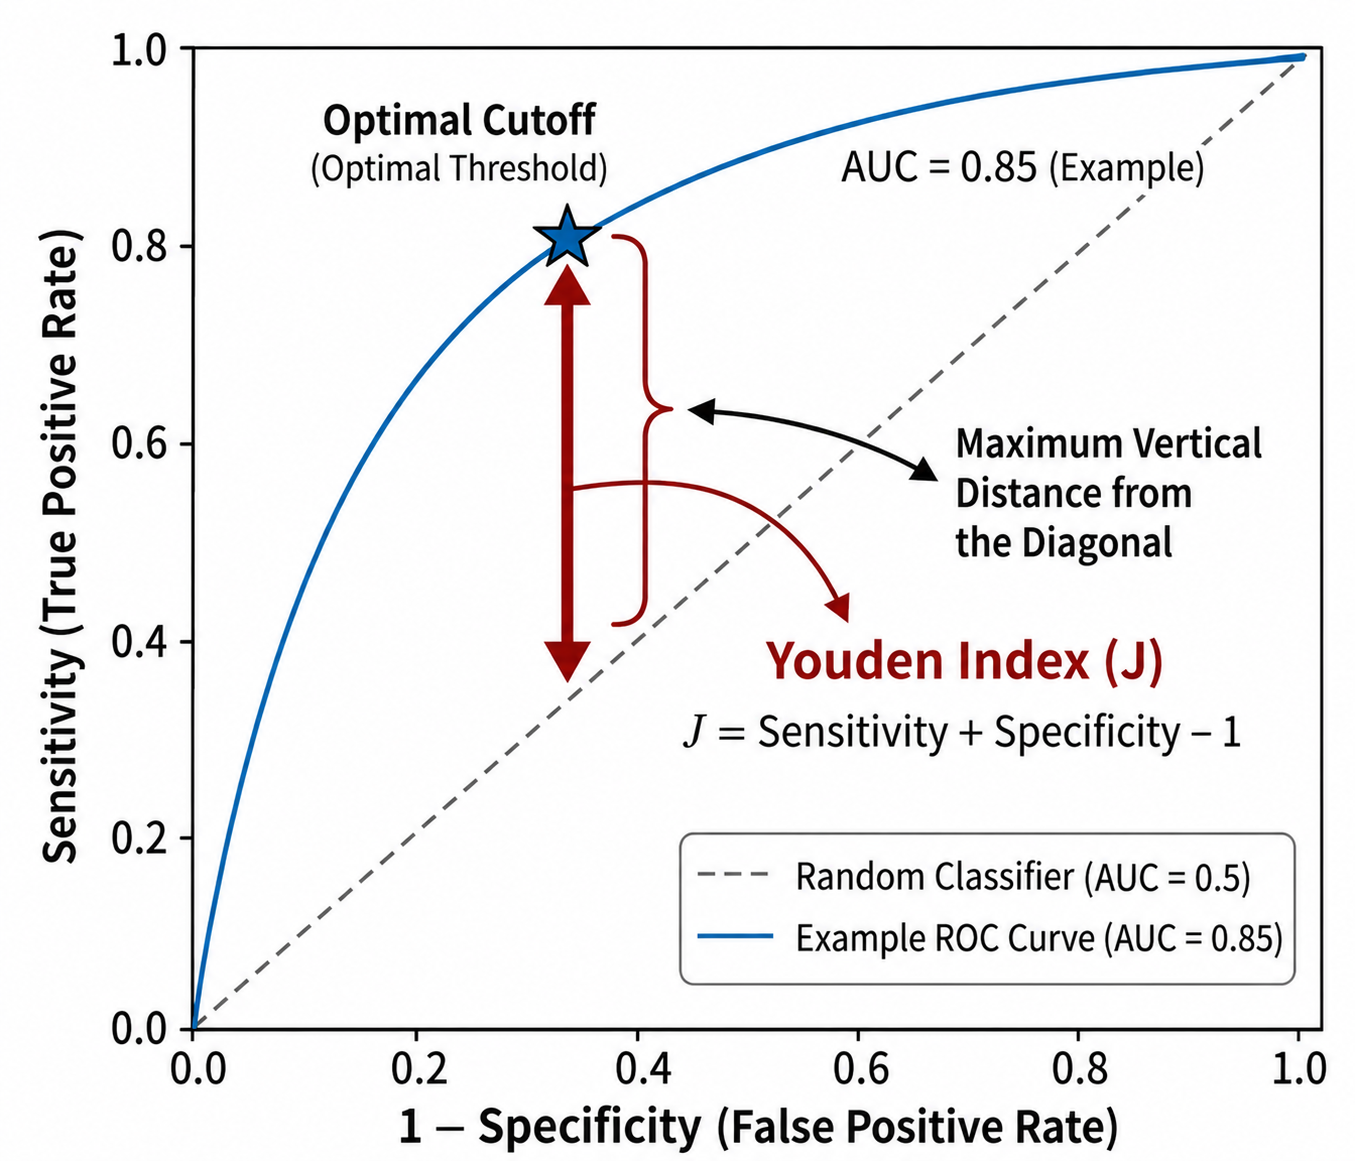
\includegraphics[width=0.55\linewidth]{figures/younden_index}
    \caption{Geometric interpretation of the Youden index on a representative ROC curve (AUC = 0.85). The index $J$ equals the maximum vertical distance from the curve to the chance diagonal; the optimal cutoff is the operating point achieving this maximum.}
    \label{fig:youden}
\end{figure}

Fig.~\ref{fig:youden} illustrates the geometric interpretation: the diagonal represents a random classifier (AUC $= 0.5$), and the starred point marks the threshold $\theta^{*}$ at which the vertical distance from the ROC curve to the diagonal is greatest.

This criterion is particularly suitable for clinical screening tasks. In medical datasets, class distributions are typically imbalanced and the cost of missing a true case (false negative) may differ substantially from the cost of a false alarm. The 0.5 default threshold---optimal only when classes are balanced and misclassification costs are equal---is therefore inappropriate. The Youden index selects the threshold that provides the best balance between sensitivity and specificity given the observed ROC curve, without requiring explicit specification of misclassification costs.

The practical estimation of $\theta^{*}$ differs between the two evaluation protocols and between the two model families, and these details are reported here for transparency.

For \emph{within-cohort LOOCV}, the out-of-fold predicted probability of every subject is accumulated across folds and $\theta^{*}$ is computed once from this pooled set of out-of-fold predictions. Because each predicted probability is generated by a model that has never seen the corresponding subject during training, this procedure is equivalent to using a validation-derived operating point in the conventional sense.

For \emph{cross-cohort transfer}, the operating point is estimated from the source cohort and reused unchanged on the 2025 test cohort. In the XGBoost feature-selection and graph-concat experiments, $\theta^{*}$ is computed from a source-cohort LOOCV pass on the 2020 training data; in the AGCN experiment, the threshold saved from the source-cohort LOOCV run is applied to the target cohort. The 2025 labels are used only for final metric computation. This avoids test-cohort threshold tuning for the reported accuracy and F1-score, while AUROC remains threshold-independent.

\subsection{Training-Termination Criteria}
\label{sec:termination}

Each model family adopts a stopping criterion appropriate to its optimization procedure.

\begin{itemize}
    \setlength{\itemsep}{0pt}
    \setlength{\parsep}{0pt}
    \setlength{\topsep}{0pt}
    \item \textbf{Logistic Regression} converges when the change in training loss between consecutive iterations falls below a predefined tolerance.
    \item \textbf{Random Forest} and \textbf{XGBoost} are trained for a fixed number of trees and nodes, respectively, as specified in Section~\ref{sec:exp_setting_hparams}.
    \item \textbf{AGCN-style model} is trained for at most 100 epochs and uses early stopping with a patience of 20 epochs without improvement in validation loss.
\end{itemize}

\subsection{Hyperparameters}
\label{sec:exp_setting_hparams}

The hyperparameters of the XGBoost and AGCN models used throughout the experiments are summarized in Tables~\ref{tab:xgboost_params} and~\ref{tab:agcn_params}.

\begin{table}[H]
    \centering
    \caption{Hyperparameter configuration for the XGBoost classifier}
    \label{tab:xgboost_params}
    \small
    \setlength{\tabcolsep}{12pt}
    \begin{tabularx}{\linewidth}{>{\raggedright\arraybackslash}X c}
        \hline
        Hyperparameter & Value \\
        \hline
        Number of estimators (\texttt{n\_estimators})       & 50 \\
        Maximum depth (\texttt{max\_depth})                  & 3 \\
        Learning rate (\texttt{learning\_rate})              & 0.1 \\
        Evaluation metric (\texttt{eval\_metric})            & logloss \\
        Random state (\texttt{random\_state})                & 42 \\
        \hline
    \end{tabularx}
\end{table}

Class imbalance across LOOCV folds is mitigated by rescaling the XGBoost positive-class weight as
\begin{equation}
    \texttt{scale\_pos\_weight} = \frac{N_{\text{negative}}}{N_{\text{positive}}}.
\end{equation}

\begin{table}[H]
    \centering
    \caption{Architectural and optimization hyperparameters for the feature-based AGCN-style framework}
    \label{tab:agcn_params}
    \small
    \setlength{\tabcolsep}{12pt}
    \begin{tabularx}{\linewidth}{>{\raggedright\arraybackslash}X >{\raggedright\arraybackslash}X}
        \hline
        Hyperparameter & Value / Configuration \\
        \hline
        Input feature dimension     & $1,764$ \\
        Graph representation        & $42$ joint nodes with $42$ descriptors per node \\
        Hidden channel dimensions   & $\{64,\,128,\,256\}$ \\
        Dropout probability         & $0.5$ \\
        Optimizer                   & AdamW \\
        Learning rate               & $0.001$ \\
        Weight decay                & $0.01$ \\
        Maximum number of epochs    & $100$ \\
        Batch size                  & $16$ \\
        Early stopping              & Patience of $20$ epochs without validation-loss improvement \\
        Loss function               & Weighted cross-entropy \\
        Number of graph nodes       & $42$ (bilateral hand joints) \\
        \hline
    \end{tabularx}
\end{table}

For AGCN-style input construction, the full bilateral feature vector is partitioned by joint. The resulting graph contains the 21 MediaPipe joints from the left hand and the 21 corresponding joints from the right hand. A fixed hand-skeleton adjacency provides the structural prior, while the same-block adaptive component learns a sample-dependent residual graph from the node features before graph convolution and global average pooling.

% Restore default spacing for subsequent chapters
\titlespacing*{\section}{0pt}{3.5ex plus 1ex minus .2ex}{2.3ex plus .2ex}
\titlespacing*{\subsection}{0pt}{3.25ex plus 1ex minus .2ex}{1.5ex plus .2ex}
\titlespacing*{\subsubsection}{0pt}{3.25ex plus 1ex minus .2ex}{1.5ex plus .2ex}
\setlength{\parskip}{10pt}


% !TeX root = ../main.tex

\chapter{Experiments and Results}
\label{chap:results}

\newcolumntype{Y}{>{\centering\arraybackslash}p{0.18\linewidth}}

This chapter presents the five experiments listed in Section~\ref{sec:roadmap}. For each experiment, the configuration follows the description in Chapter~\ref{chap:methods}, and detailed numerical results are reported as tables and ROC curves to support the accompanying analysis.

\section{Experiment~1: Thumb-Tip Features vs.\ Bilateral Hand Joint Features}
\label{sec:exp1}

\subsection{Configuration}

In Experiment~1, two feature subsets are compared as input to three classical classifiers:
\begin{itemize}
    \item \textbf{Thumb-tip features.} Frequency, clarity, and amplitude features derived only from the thumb-tip trajectory (joint~4). The thumb tip is visually the most-displaced joint during pronation-supination and therefore a natural single-joint baseline.
    \item \textbf{Bilateral hand joint features.} The full 1{,}764-dimensional vector of features extracted from all 21 joints of both hands.
\end{itemize}

For each feature subset, Logistic Regression, Random Forest, and XGBoost are trained and evaluated under LOOCV on each cohort, and additionally under the 2020-to-2025 cross-cohort transfer protocol.

\subsection{Results}

Table~\ref{tab:thumb_model_comparison} reports the within-cohort LOOCV performance of the three classifiers on thumb-tip features. Table~\ref{tab:bilateral_model_comparison} reports the corresponding within-cohort results on bilateral hand-joint features. Figures~\ref{fig:thumb_roc_comparison} and~\ref{fig:bilateral_roc_comparison} show the corresponding ROC curves under both LOOCV and cross-cohort protocols. The explicit cross-cohort metrics (train on 2020, test on 2025) are summarized in Tables~\ref{tab:thumb_cross_dataset} and~\ref{tab:bilateral_cross_dataset}.

\begin{table}[H]
    \centering
    \caption{Within-cohort LOOCV performance of three classifiers on thumb-tip features}
    \label{tab:thumb_model_comparison}
    \small
    \setlength{\tabcolsep}{4pt}
    \begin{tabularx}{\linewidth}{>{\raggedright\arraybackslash}XYYY}
        \hline
        Model & \shortstack{AUROC\\(2020/2025)} & \shortstack{Accuracy\\(2020/2025)} & \shortstack{F1-score\\(2020/2025)} \\
        \hline
        Logistic Regression & 0.75 / 0.67 & 0.68 / 0.77 & 0.61 / 0.56 \\
        Random Forest       & 0.77 / 0.69 & 0.74 / 0.69 & 0.65 / 0.49 \\
        XGBoost             & 0.77 / 0.61 & 0.72 / 0.71 & 0.62 / 0.41 \\
        \hline
    \end{tabularx}
\end{table}

\begin{table}[H]
    \centering
    \caption{Within-cohort LOOCV performance of three classifiers on bilateral hand joint features}
    \label{tab:bilateral_model_comparison}
    \small
    \setlength{\tabcolsep}{4pt}
    \begin{tabularx}{\linewidth}{>{\raggedright\arraybackslash}XYYY}
        \hline
        Model & \shortstack{AUROC\\(2020/2025)} & \shortstack{Accuracy\\(2020/2025)} & \shortstack{F1-score\\(2020/2025)} \\
        \hline
        Logistic Regression & 0.81 / 0.67 & 0.79 / 0.80 & 0.67 / 0.50 \\
        Random Forest       & 0.82 / 0.71 & 0.73 / 0.71 & 0.66 / 0.51 \\
        XGBoost             & 0.77 / 0.62 & 0.74 / 0.73 & 0.61 / 0.47 \\
        \hline
    \end{tabularx}
\end{table}

\begin{table}[H]
    \centering
    \caption{Cross-cohort evaluation on thumb-tip features (train on 2020, test on 2025)}
    \label{tab:thumb_cross_dataset}
    \small
    \setlength{\tabcolsep}{4pt}
    \begin{tabularx}{\linewidth}{>{\raggedright\arraybackslash}XYYY}
        \hline
        Model & AUROC & Accuracy & F1-score \\
        \hline
        Logistic Regression & 0.63 & 0.52 & 0.46 \\
        Random Forest       & 0.71 & 0.51 & 0.46 \\
        XGBoost             & 0.71 & 0.51 & 0.44 \\
        \hline
    \end{tabularx}
\end{table}

\begin{table}[H]
    \centering
    \caption{Cross-cohort evaluation on bilateral hand joint features (train on 2020, test on 2025)}
    \label{tab:bilateral_cross_dataset}
    \small
    \setlength{\tabcolsep}{4pt}
    \begin{tabularx}{\linewidth}{>{\raggedright\arraybackslash}XYYY}
        \hline
        Model & AUROC & Accuracy & F1-score \\
        \hline
        Logistic Regression & 0.51 & 0.47 & 0.34 \\
        Random Forest       & 0.68 & 0.35 & 0.41 \\
        XGBoost             & 0.69 & 0.46 & 0.42 \\
        \hline
    \end{tabularx}
\end{table}

\begin{figure}[H]
    \centering
    \begin{subfigure}[b]{0.32\textwidth}
        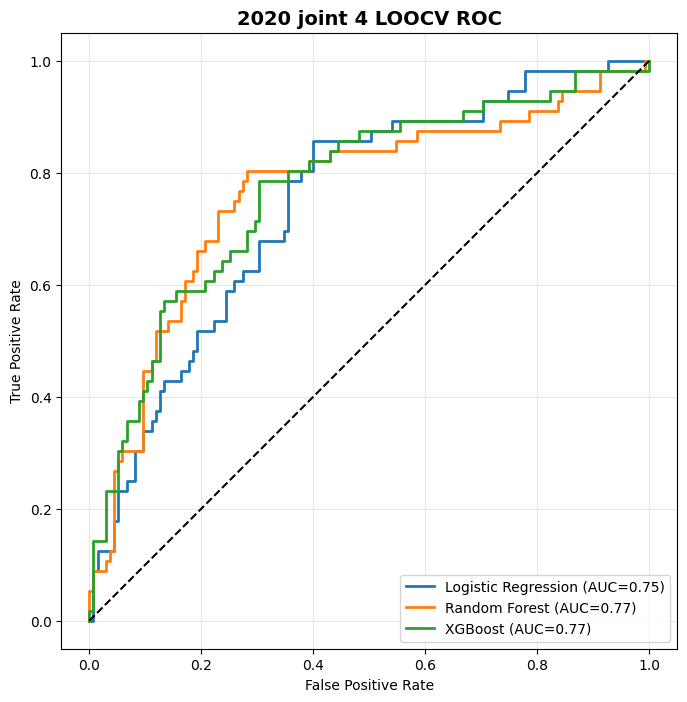
\includegraphics[width=\textwidth]{figures/2020_joint4.png}
        \caption{2020 (LOOCV) test}
        \label{fig:thumb_roc_2020}
    \end{subfigure}
    \hfill
    \begin{subfigure}[b]{0.32\textwidth}
        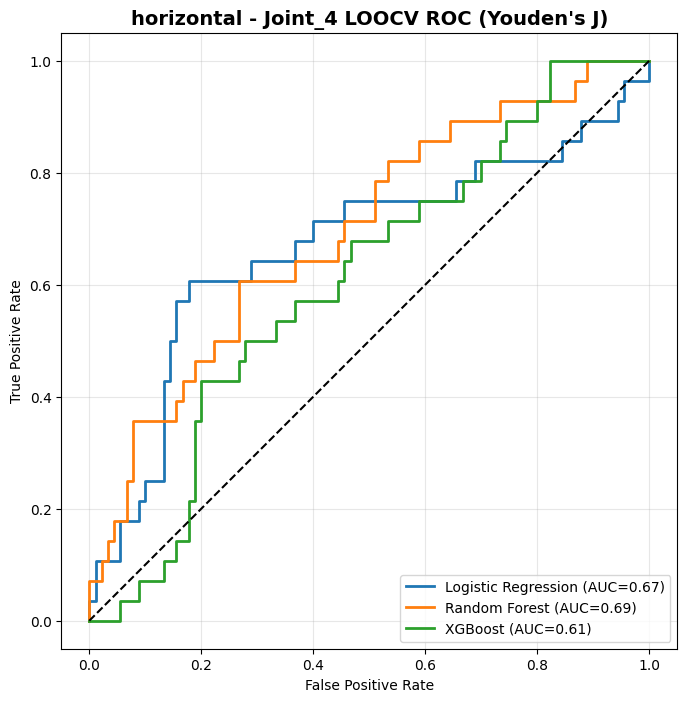
\includegraphics[width=\textwidth]{figures/2025_joint4.png}
        \caption{2025 (LOOCV)}
        \label{fig:thumb_roc_2025}
    \end{subfigure}
    \hfill
    \begin{subfigure}[b]{0.32\textwidth}
        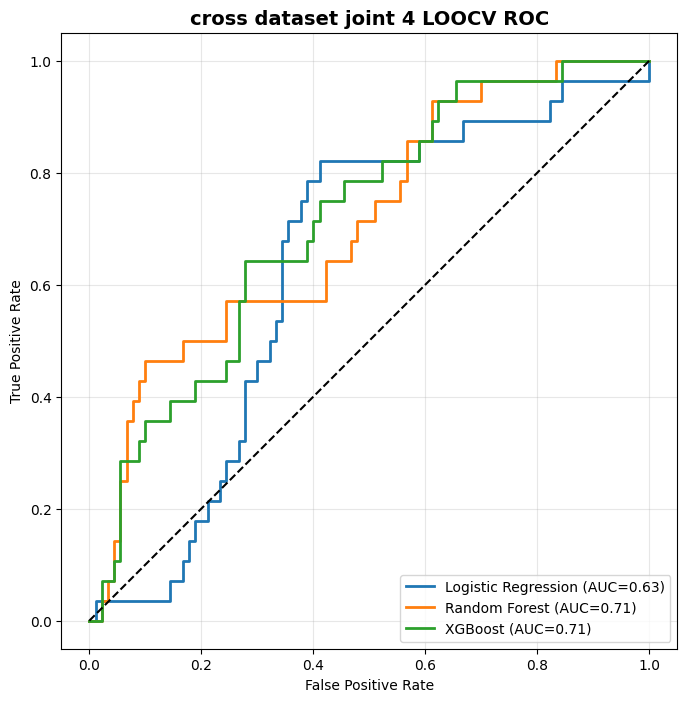
\includegraphics[width=\textwidth]{figures/cross_joint4.png}
        \caption{Cross-cohort}
        \label{fig:thumb_roc_cross}
    \end{subfigure}
    \caption{ROC curves on thumb-tip features under LOOCV and cross-cohort transfer.}
    \label{fig:thumb_roc_comparison}
\end{figure}

\begin{figure}[H]
    \centering
    \begin{subfigure}[t]{0.32\textwidth}
        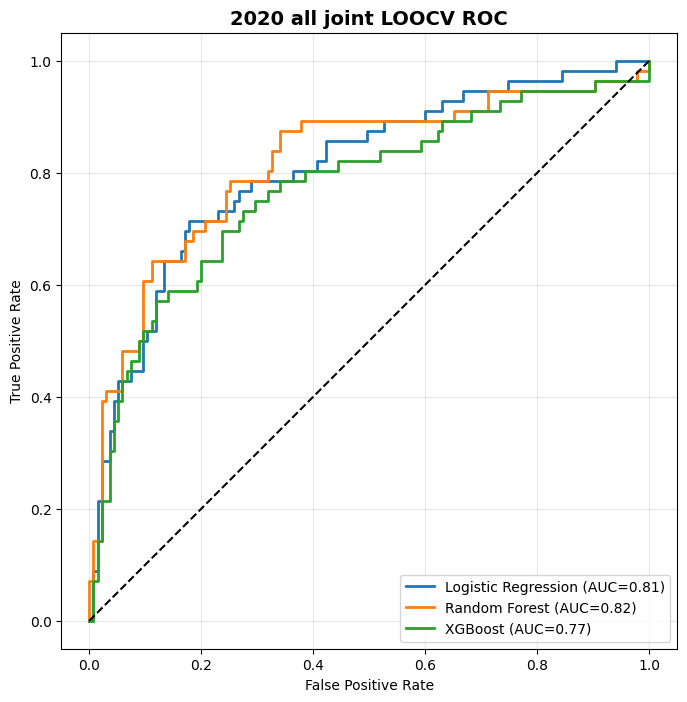
\includegraphics[width=\textwidth]{figures/2020_All_Joints.png}
        \caption{2020 (LOOCV)}
        \label{fig:bilateral_roc_2020}
    \end{subfigure}
    \hfill
    \begin{subfigure}[t]{0.32\textwidth}
        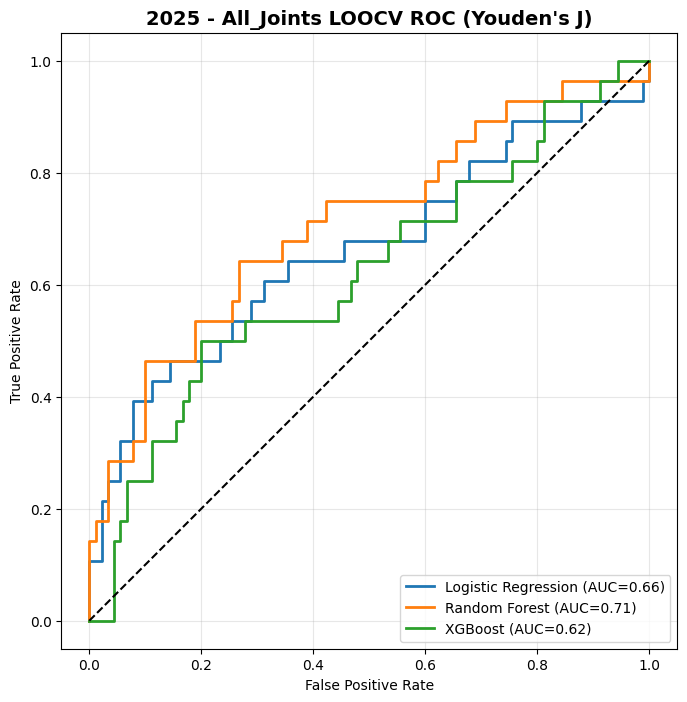
\includegraphics[width=\textwidth]{figures/2025_All_Joints.png}
        \caption{2025 (LOOCV)}
        \label{fig:bilateral_roc_2025}
    \end{subfigure}
    \hfill
    \begin{subfigure}[t]{0.32\textwidth}
        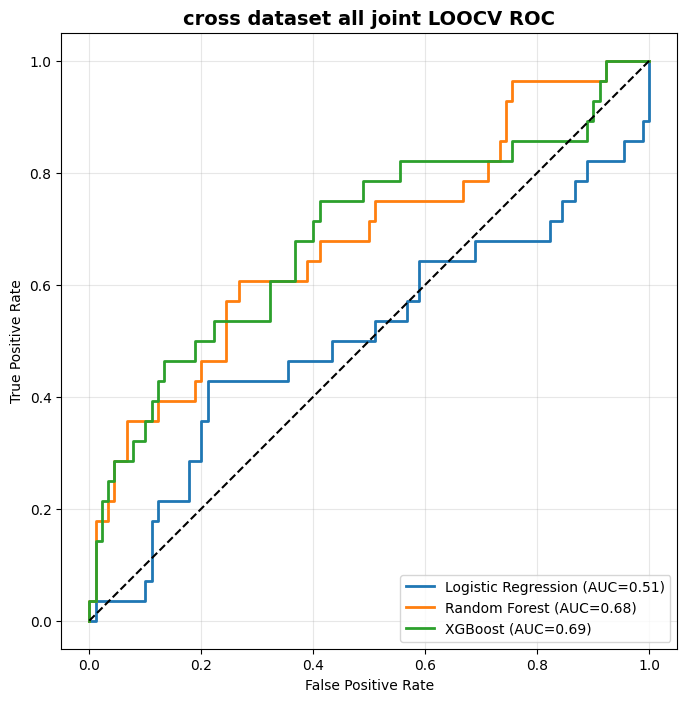
\includegraphics[width=\textwidth]{figures/cross_All_joints.png}
        \caption{Cross-cohort}
        \label{fig:bilateral_roc_cross}
    \end{subfigure}
    \caption{ROC curves on bilateral hand joint features under LOOCV and cross-cohort transfer.}
    \label{fig:bilateral_roc_comparison}
\end{figure}

\subsection{Observation}

Under LOOCV, performance on the 2020 and 2025 cohorts is broadly comparable across the two feature subsets and the three classifier families: thumb-tip features and bilateral features yield similar AUROC values, with no single classifier dominating in both cohorts simultaneously. In the cross-cohort transfer setting, however, XGBoost emerges as the most stable model in terms of AUROC, retaining $0.71$ on thumb-tip features and $0.69$ on bilateral features. This observation motivates the choice of XGBoost as the default downstream classifier for all subsequent experiments.

\section{Experiment~2: Feature Selection on Bilateral Hand Joint Features with XGBoost}
\label{sec:exp2}

\subsection{Configuration}

Experiment~2 builds on the bilateral feature subset of Experiment~1 by inserting an explicit feature-selection stage in front of the XGBoost classifier. The three feature-selection strategies introduced in Section~\ref{sec:fs} are compared: ANOVA F-value (\texttt{SelectKBest}), L1-regularized Logistic Regression, and XGBoost gain-based importance. The downstream classifier remains XGBoost. Feature selection is re-run inside every LOOCV training fold.

\subsection{Results}

Table~\ref{tab:fs_xgb_bilateral_comparison} reports the within-cohort LOOCV performance of the three feature-selection methods combined with XGBoost. Figure~\ref{fig:fs_bilateral_roc_comparison} shows the corresponding ROC curves, and Figure~\ref{fig:fs_bilateral_scatter_comparison} shows two-dimensional scatter plots of the most discriminative selected features. The cross-cohort transfer results are summarized in Table~\ref{tab:fs_bilateral_cross_dataset}.

\begin{table}[H]
    \centering
    \caption{Feature selection on bilateral features combined with XGBoost (LOOCV)}
    \label{tab:fs_xgb_bilateral_comparison}
    \small
    \setlength{\tabcolsep}{4pt}
    \begin{tabularx}{\linewidth}{>{\raggedright\arraybackslash}XYYY}
        \hline
        Method & \shortstack{AUROC\\(2020/2025)} & \shortstack{Accuracy\\(2020/2025)} & \shortstack{F1-score\\(2020/2025)} \\
        \hline
        ANOVA + XGBoost              & 0.74 / 0.62 & 0.76 / 0.48 & 0.64 / 0.45 \\
        L1-Logistic + XGBoost        & 0.74 / 0.57 & 0.80 / 0.62 & 0.61 / 0.43 \\
        XGB Importance + XGBoost     & 0.74 / 0.69 & 0.78 / 0.73 & 0.60 / 0.54 \\
        \hline
    \end{tabularx}
\end{table}

\begin{table}[H]
    \centering
    \caption{Cross-cohort evaluation of feature selection on bilateral features with XGBoost (train on 2020, test on 2025)}
    \label{tab:fs_bilateral_cross_dataset}
    \small
    \setlength{\tabcolsep}{4pt}
    \begin{tabularx}{\linewidth}{>{\raggedright\arraybackslash}XYYY}
        \hline
        Method & AUROC & Accuracy & F1-score \\
        \hline
        ANOVA + XGBoost              & 0.68 & 0.52 & 0.42 \\
        L1-Logistic + XGBoost        & 0.68 & 0.66 & 0.46 \\
        XGB Importance + XGBoost     & 0.65 & 0.56 & 0.41 \\
        \hline
    \end{tabularx}
\end{table}

\begin{figure}[H]
    \centering
    \begin{subfigure}[t]{0.32\textwidth}
        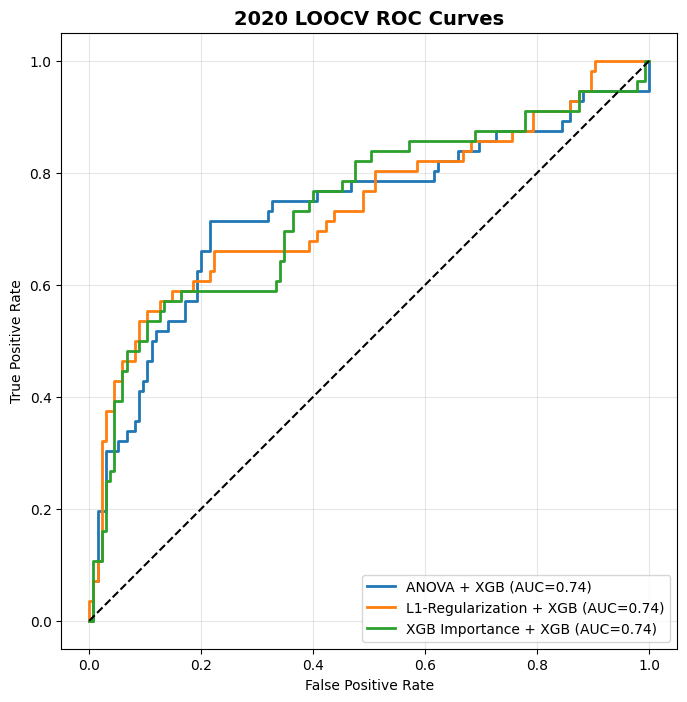
\includegraphics[width=\textwidth]{figures/2020_fs_bilateral.png}
        \caption{2020 (LOOCV)}
        \label{fig:fs_bilateral_roc_2020}
    \end{subfigure}
    \hfill
    \begin{subfigure}[t]{0.32\textwidth}
        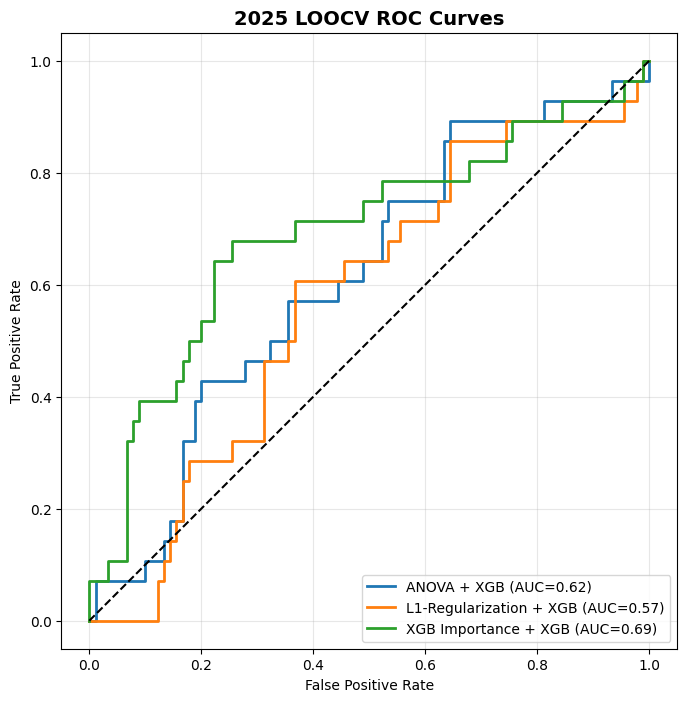
\includegraphics[width=\textwidth]{figures/2025_fs_bilateral.png}
        \caption{2025 (LOOCV)}
        \label{fig:fs_bilateral_roc_2025}
    \end{subfigure}
    \hfill
    \begin{subfigure}[t]{0.32\textwidth}
        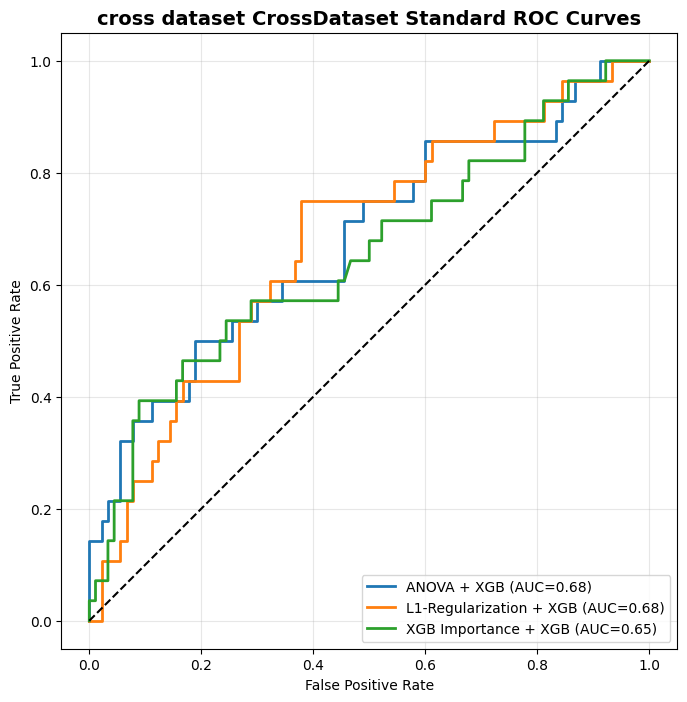
\includegraphics[width=\textwidth]{figures/cross_fs_bilateral.png}
        \caption{Cross-cohort}
        \label{fig:fs_bilateral_roc_cross}
    \end{subfigure}
    \caption{ROC curves of feature selection on bilateral features combined with XGBoost.}
    \label{fig:fs_bilateral_roc_comparison}
\end{figure}

\begin{figure}[H]
    \centering
    \begin{subfigure}[t]{0.32\textwidth}
        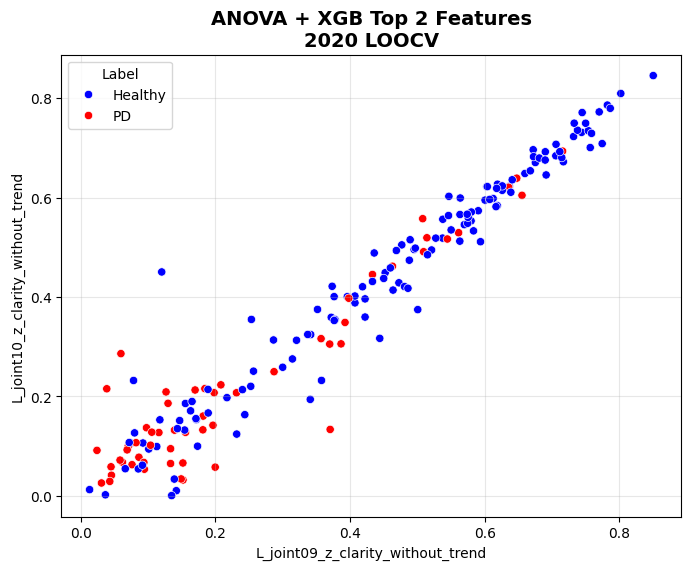
\includegraphics[width=\textwidth]{figures/2020_anova_fs_scatter.png}
        \caption{ANOVA, 2020}
    \end{subfigure}
    \hfill
    \begin{subfigure}[t]{0.32\textwidth}
        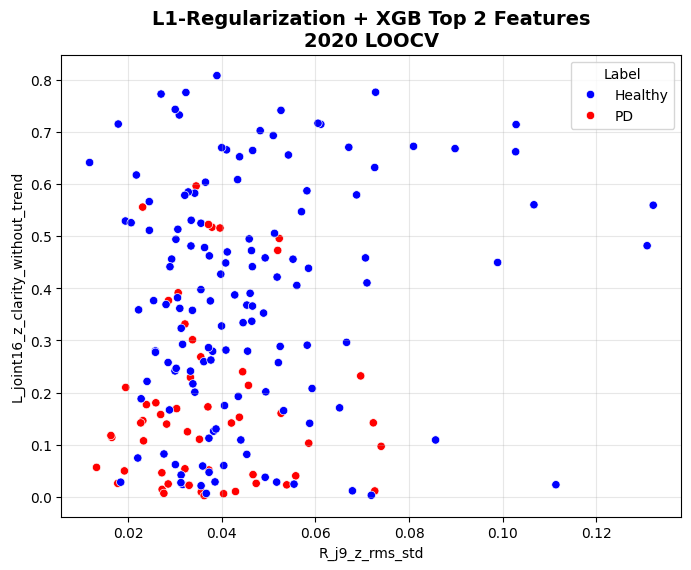
\includegraphics[width=\textwidth]{figures/2020_l1_fs_scatter.png}
        \caption{L1-Logistic, 2020}
    \end{subfigure}
    \hfill
    \begin{subfigure}[t]{0.32\textwidth}
        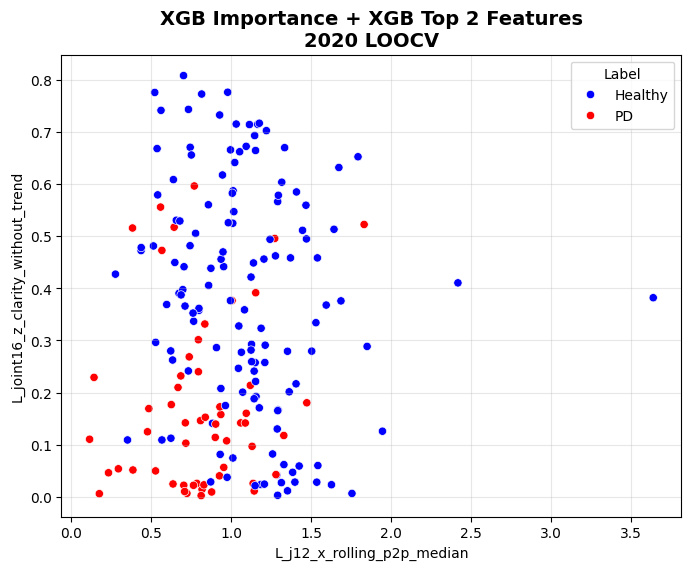
\includegraphics[width=\textwidth]{figures/2020_xgbimp_fs_scatter.png}
        \caption{XGB Importance, 2020}
    \end{subfigure}

    \vspace{0.2em}

    \begin{subfigure}[t]{0.32\textwidth}
        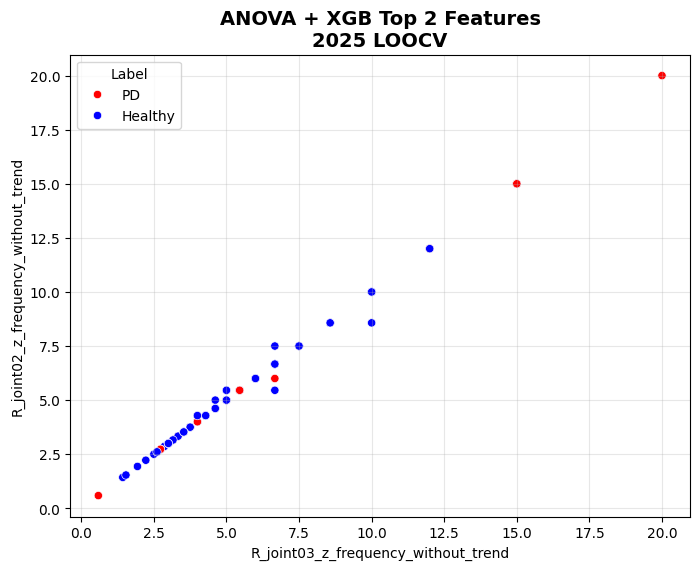
\includegraphics[width=\textwidth]{figures/2025_anova_fs_scatter.png}
        \caption{ANOVA, 2025}
    \end{subfigure}
    \hfill
    \begin{subfigure}[t]{0.32\textwidth}
        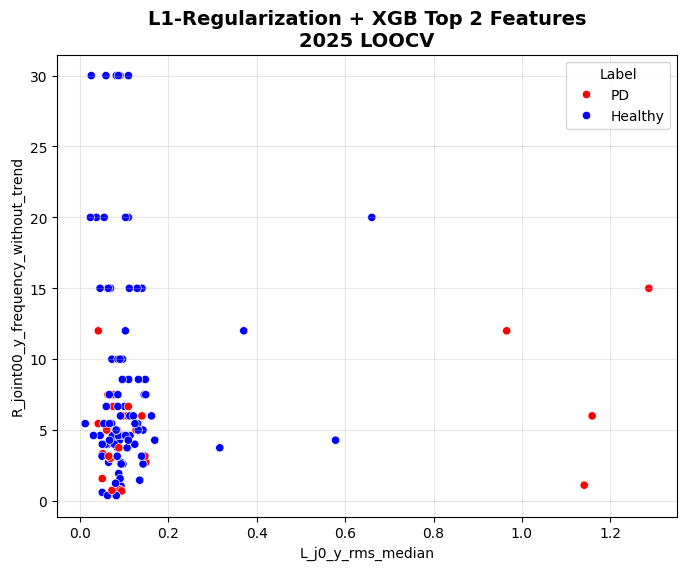
\includegraphics[width=\textwidth]{figures/2025_l1_fs_scatter.png}
        \caption{L1-Logistic, 2025}
    \end{subfigure}
    \hfill
    \begin{subfigure}[t]{0.32\textwidth}
        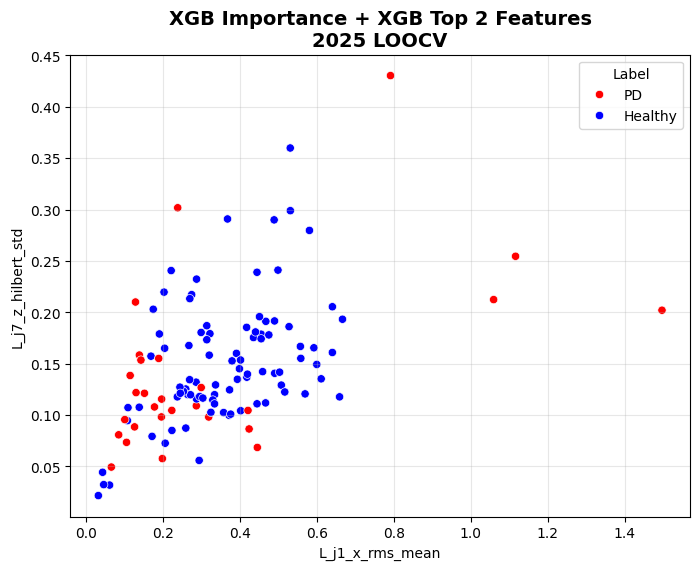
\includegraphics[width=\textwidth]{figures/2025_xgbimp_fs_scatter.png}
        \caption{XGB Importance, 2025}
    \end{subfigure}
    \caption{Scatter plots of the most discriminative selected features for the three feature-selection methods on bilateral features (PD vs healthy).}
    \label{fig:fs_bilateral_scatter_comparison}
\end{figure}

\subsection{Top-10 Hand-Side Distribution}

To investigate which hand contributes most of the discriminative signal, the top-10 selected features are first aggregated across LOOCV folds for each feature-selection method. The counts in Table~\ref{tab:fs_topk_hand_distribution} then sum these top-10 lists across the three methods, so each cohort contributes 30 selected-feature slots rather than a single set of 10 features.

\begin{table}[H]
    \centering
    \caption{Aggregated distribution of top-10 selected features across the three feature-selection methods}
    \label{tab:fs_topk_hand_distribution}
    \small
    \setlength{\tabcolsep}{8pt}
    \begin{tabularx}{\linewidth}{>{\raggedright\arraybackslash}X c c}
        \hline
        Cohort & Right-hand count & Left-hand count \\
        \hline
        2020 & 5  & 25 \\
        2025 & 11 & 19 \\
        \hline
    \end{tabularx}
\end{table}

\subsection{Observation}

All three feature-selection methods reach the same AUROC of $0.74$ on the 2020 cohort. On the 2025 cohort, XGBoost Importance yields the strongest within-cohort generalization, with the highest AUROC ($0.69$), accuracy ($0.73$), and F1-score ($0.54$). In the cross-cohort transfer setting, ANOVA and L1-Logistic feature selection retain the highest AUROC of $0.68$, but the threshold-dependent accuracy and F1-score remain modest, indicating that transfer across cohorts is still difficult.

The hand-side distribution in Table~\ref{tab:fs_topk_hand_distribution} reveals a consistent left-versus-right asymmetry across the 30 selected-feature slots: the left hand contributes $25{:}5$ on the 2020 cohort and $19{:}11$ on the 2025 cohort. This observation directly motivates Experiment~3.

\section{Experiment~3: Left-Hand-Only vs.\ Right-Hand-Only Feature Selection with XGBoost}
\label{sec:exp3}

\subsection{Configuration}

Experiment~3 repeats the feature-selection-plus-XGBoost pipeline of Experiment~2 on three feature subsets: the left-hand-only subset, the right-hand-only subset, and the bilateral subset (the latter is included for reference). All other settings, including LOOCV protocol and cross-cohort transfer, are identical to Experiment~2.

\subsection{Results}

Tables~\ref{tab:fs_xgb_right_hand_comparison} and~\ref{tab:fs_xgb_left_hand_comparison} report the within-cohort LOOCV performance for the right and left hand respectively, and Figure~\ref{fig:fs_hand_roc_comparison} shows the corresponding ROC curves. The cross-cohort transfer results are summarized in Table~\ref{tab:fs_lr_hand_cross_dataset}.

\begin{table}[H]
    \centering
    \caption{Right-hand-only feature selection combined with XGBoost (LOOCV)}
    \label{tab:fs_xgb_right_hand_comparison}
    \small
    \setlength{\tabcolsep}{4pt}
    \begin{tabularx}{\linewidth}{>{\raggedright\arraybackslash}XYYY}
        \hline
        Method & \shortstack{AUROC\\(2020/2025)} & \shortstack{Accuracy\\(2020/2025)} & \shortstack{F1-score\\(2020/2025)} \\
        \hline
        ANOVA + XGBoost              & 0.57 / 0.67 & 0.66 / 0.69 & 0.40 / 0.45 \\
        L1-Logistic + XGBoost        & 0.70 / 0.77 & 0.62 / 0.64 & 0.55 / 0.53 \\
        XGB Importance + XGBoost     & 0.68 / 0.56 & 0.66 / 0.70 & 0.53 / 0.36 \\
        \hline
    \end{tabularx}
\end{table}

\begin{table}[H]
    \centering
    \caption{Left-hand-only feature selection combined with XGBoost (LOOCV)}
    \label{tab:fs_xgb_left_hand_comparison}
    \small
    \setlength{\tabcolsep}{4pt}
    \begin{tabularx}{\linewidth}{>{\raggedright\arraybackslash}XYYY}
        \hline
        Method & \shortstack{AUROC\\(2020/2025)} & \shortstack{Accuracy\\(2020/2025)} & \shortstack{F1-score\\(2020/2025)} \\
        \hline
        ANOVA + XGBoost              & 0.74 / 0.53 & 0.76 / 0.63 & 0.64 / 0.39 \\
        L1-Logistic + XGBoost        & 0.78 / 0.63 & 0.79 / 0.70 & 0.66 / 0.44 \\
        XGB Importance + XGBoost     & 0.76 / 0.75 & 0.82 / 0.81 & 0.65 / 0.63 \\
        \hline
    \end{tabularx}
\end{table}

\begin{table}[H]
    \centering
    \caption{Cross-cohort evaluation of right- and left-hand-only feature selection with XGBoost (train on 2020, test on 2025)}
    \label{tab:fs_lr_hand_cross_dataset}
    \small
    \setlength{\tabcolsep}{4pt}
    \begin{tabularx}{\linewidth}{>{\raggedleft\arraybackslash}p{0.15\linewidth}XYYY}
        \hline
        & Method & AUROC & Accuracy & F1-score \\
        \hline
        \multirow{3}{*}{Right hand} & ANOVA + XGBoost           & 0.68 & 0.66 & 0.41 \\
                                    & L1-Logistic + XGBoost     & 0.62 & 0.42 & 0.38 \\
                                    & XGB Importance + XGBoost  & 0.65 & 0.52 & 0.39 \\
        \hline
        \multirow{3}{*}{Left hand}  & ANOVA + XGBoost           & 0.68 & 0.52 & 0.42 \\
                                    & L1-Logistic + XGBoost     & 0.64 & 0.63 & 0.41 \\
                                    & XGB Importance + XGBoost  & 0.66 & 0.65 & 0.47 \\
        \hline
    \end{tabularx}
\end{table}

\begin{figure}[H]
    \centering
    \begin{subfigure}[t]{0.32\textwidth}
        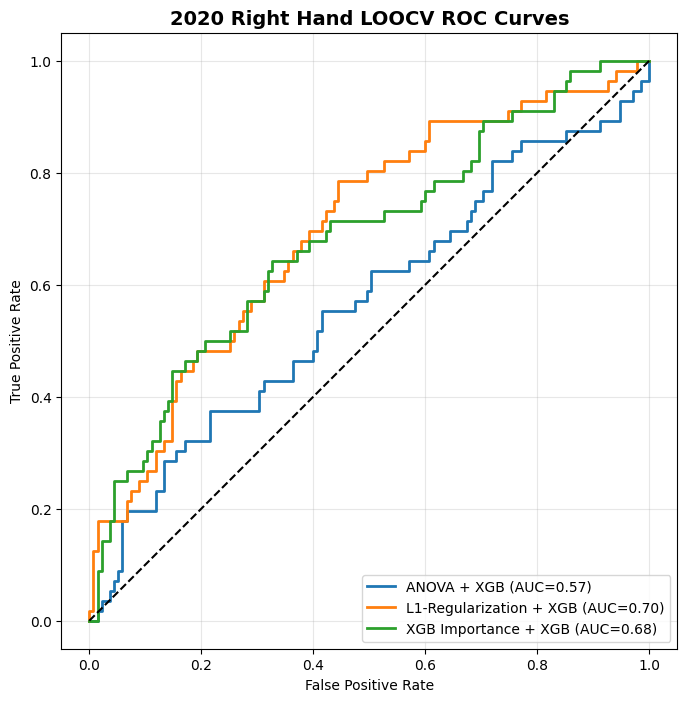
\includegraphics[width=\textwidth]{figures/2020_right_hand_fs.png}
        \caption{Right hand, 2020}
    \end{subfigure}
    \hfill
    \begin{subfigure}[t]{0.32\textwidth}
        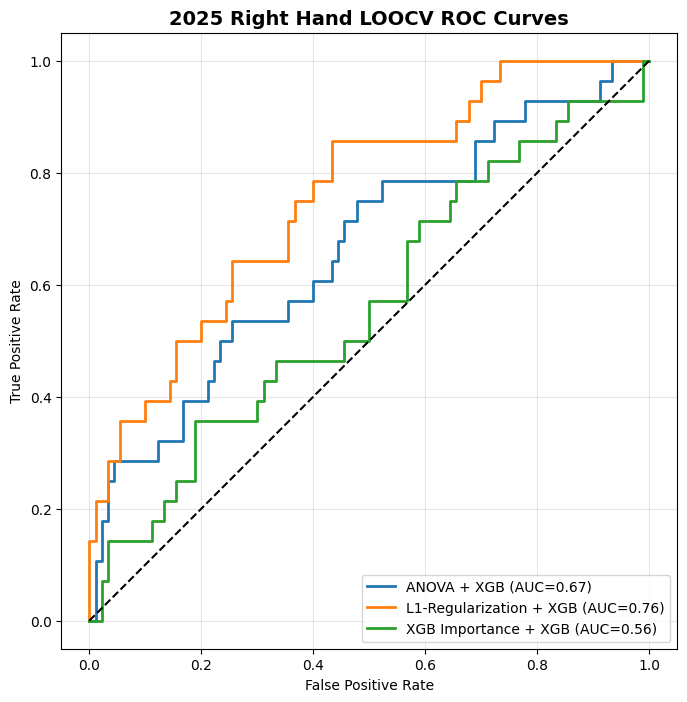
\includegraphics[width=\textwidth]{figures/2025_right_hand_fs.png}
        \caption{Right hand, 2025}
    \end{subfigure}
    \hfill
    \begin{subfigure}[t]{0.32\textwidth}
        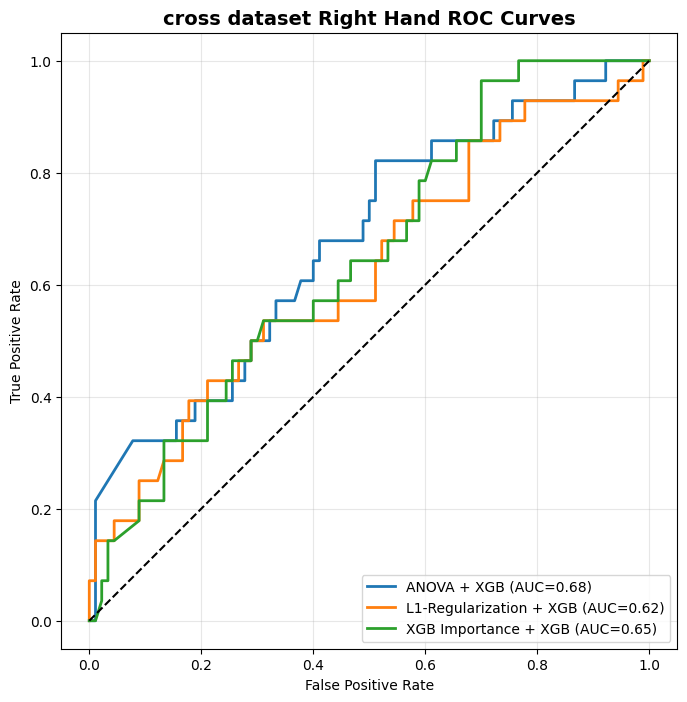
\includegraphics[width=\textwidth]{figures/cross_right_hand_fs.png}
        \caption{Right hand, cross-cohort}
    \end{subfigure}

    \vspace{0.2em}

    \begin{subfigure}[t]{0.32\textwidth}
        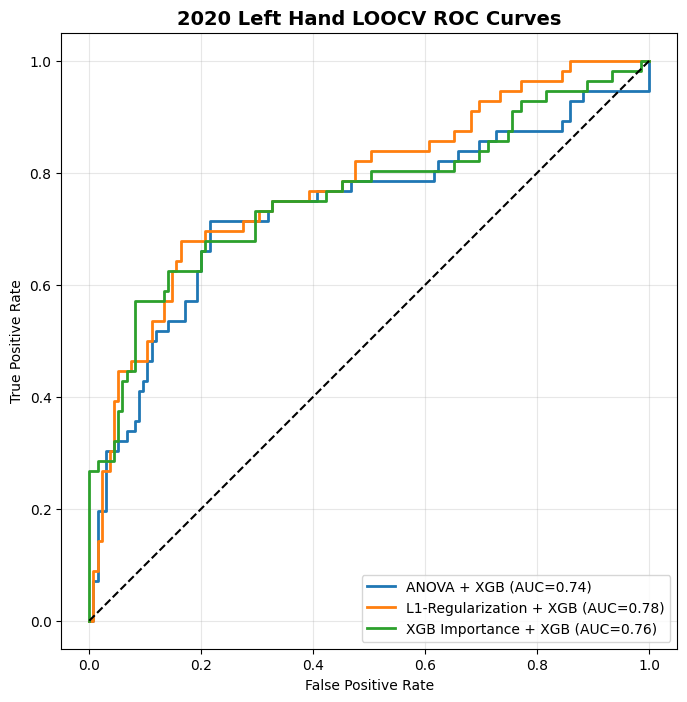
\includegraphics[width=\textwidth]{figures/2020_left_hand_fs.png}
        \caption{Left hand, 2020}
    \end{subfigure}
    \hfill
    \begin{subfigure}[t]{0.32\textwidth}
        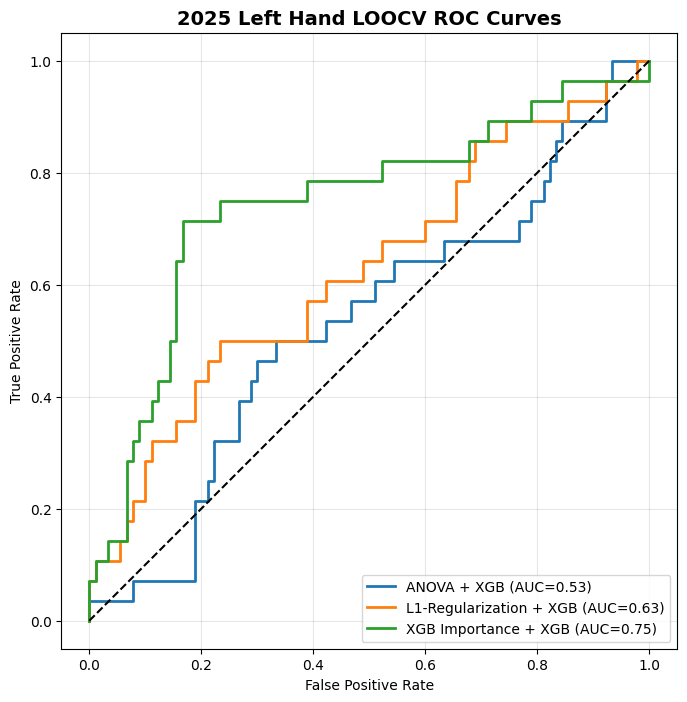
\includegraphics[width=\textwidth]{figures/2025_left_hand_fs.png}
        \caption{Left hand, 2025}
    \end{subfigure}
    \hfill
    \begin{subfigure}[t]{0.32\textwidth}
        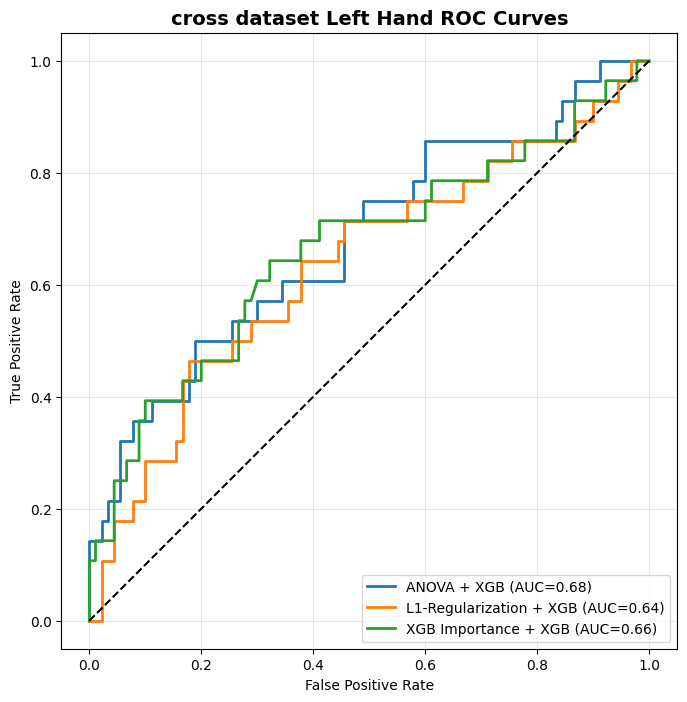
\includegraphics[width=\textwidth]{figures/cross_left_hand_fs.png}
        \caption{Left hand, cross-cohort}
    \end{subfigure}
    \caption{ROC curves of feature selection combined with XGBoost on right-hand-only and left-hand-only features.}
    \label{fig:fs_hand_roc_comparison}
\end{figure}

\subsection{Observation}

The left-hand XGB Importance + XGBoost configuration is the strongest single-hand baseline, reaching AUROCs of $0.76$ and $0.75$ on the 2020 and 2025 cohorts respectively, with accuracies of $0.82$ and $0.81$. The advantage is most consistent for the XGB-importance selector: it outperforms the corresponding right-hand configuration in both cohorts and also yields the highest cross-cohort F1-score among single-hand models. This pattern, together with the left-heavy top-feature distribution observed in Experiment~2, is consistent with a scenario in which the dominant hand retains more motor reserve and therefore shows less feature separation, while the non-dominant hand exhibits earlier and more detectable kinematic decline. However, this interpretation should be treated with caution. Because individual handedness was not recorded, it cannot be established that the left hand was non-dominant for the majority of subjects in either cohort. The observed asymmetry may alternatively reflect population-level differences in how PD pathology progresses across the two sides, recording-specific confounds, or the particular joints and features selected by the XGB importance method. The finding is therefore reported as an empirical left-versus-right asymmetry in feature discriminability rather than as confirmatory evidence for the motor-reserve hypothesis.

\section{Experiment~4: Bilateral Features Plus Graph-Aggregated Joint-Correlation Features}
\label{sec:exp4}

\subsection{Configuration}

Experiment~4 evaluates whether the 203-dimensional graph-aggregated joint-correlation descriptor (Section~\ref{sec:joint_corr_corr}) adds discriminative value on top of the bilateral kinematic features. The bilateral feature vector is extended from 1,764 to 1,967 dimensions by appending the graph descriptor, which encodes inter-joint feature-profile similarity via a Ledoit-Wolf shrinkage correlation matrix, one step of GCN-style aggregation, node-level pooling statistics, bilateral asymmetry, and block-level intra/inter-hand coupling statistics. The three feature-selection strategies are then applied to reduce this extended space, and XGBoost is used as the downstream classifier. Two baselines are kept for comparison: the strongest single-side model from Experiment~3 (left-hand XGB Importance) and the strongest bilateral model from Experiment~2 (bilateral XGB Importance).

\subsection{Results}

Table~\ref{tab:correlation_within_cohort} reports the within-cohort LOOCV performance and Table~\ref{tab:correlation_cross_dataset} reports the cross-cohort transfer results.

\begin{table}[H]
    \centering
    \caption{Within-cohort LOOCV performance with graph-aggregated joint-correlation features added to the bilateral feature set}
    \label{tab:correlation_within_cohort}
    \small
    \setlength{\tabcolsep}{4pt}
    \begin{tabularx}{\linewidth}{>{\raggedright\arraybackslash}XYYY}
        \hline
        Method & \shortstack{AUROC\\(2020/2025)} & \shortstack{Accuracy\\(2020/2025)} & \shortstack{F1-score\\(2020/2025)} \\
        \hline
        Left-hand XGB Importance (baseline)         & 0.76 / 0.75 & 0.82 / 0.81 & 0.65 / 0.63 \\
        Bilateral XGB Importance (baseline)         & 0.74 / 0.69 & 0.78 / 0.73 & 0.60 / 0.54 \\
        Graph-Corr + ANOVA + XGBoost               & 0.74 / 0.61 & 0.77 / 0.63 & 0.63 / 0.44 \\
        Graph-Corr + L1-Logistic + XGBoost         & 0.72 / 0.56 & 0.79 / 0.60 & 0.62 / 0.42 \\
        Graph-Corr + XGB Importance + XGBoost      & 0.73 / 0.66 & 0.78 / 0.61 & 0.60 / 0.48 \\
        \hline
    \end{tabularx}
\end{table}

\begin{table}[H]
    \centering
    \caption{Cross-cohort evaluation with graph-aggregated joint-correlation features (train on 2020, test on 2025)}
    \label{tab:correlation_cross_dataset}
    \small
    \setlength{\tabcolsep}{4pt}
    \begin{tabularx}{\linewidth}{>{\raggedright\arraybackslash}XYYY}
        \hline
        Method & AUROC & Accuracy & F1-score \\
        \hline
        Left-hand XGB Importance (baseline)         & 0.66 & 0.65 & 0.47 \\
        Bilateral XGB Importance (baseline)         & 0.65 & 0.56 & 0.41 \\
        Graph-Corr + ANOVA + XGBoost               & 0.68 & 0.56 & 0.45 \\
        Graph-Corr + L1-Logistic + XGBoost         & 0.65 & 0.62 & 0.44 \\
        Graph-Corr + XGB Importance + XGBoost      & 0.67 & 0.58 & 0.45 \\
        \hline
    \end{tabularx}
\end{table}

\subsection{Observation}

Adding the 203-dimensional graph-aggregated joint-correlation descriptor does \emph{not} produce a consistent improvement over the strongest baselines. Within cohort, the best augmented configuration only matches the bilateral baseline (AUROC $0.74$) on the 2020 cohort and reaches AUROC $0.66$ on the 2025 cohort, both below the left-hand-only baseline (AUROC $0.75$). In the cross-cohort transfer setting, the ANOVA- and XGB-based augmented configurations yield AUROC of $0.68$ and $0.67$ respectively, marginally above the two baselines ($0.65$--$0.66$), but the L1-regularised configuration ($0.65$) does not improve over the bilateral baseline. Accuracy and F1-score show no consistent gain. We interpret this as evidence that, once autocorrelation and amplitude descriptors are in place, the additional graph-structured inter-joint correlation carries limited incremental discriminative information.

\section{Experiment~5: Adaptive Graph Convolutional Network}
\label{sec:exp5}

\subsection{Configuration}

Experiment~5 evaluates the feature-based AGCN-style model described in Section~\ref{sec:joint_corr_agcn}. The model uses the same 1,764-dimensional bilateral kinematic feature vector as the preceding feature-based experiments, but reorganises it as a 42-node joint graph rather than treating it as a flat tabular vector. The adaptive graph is derived from the layer-wise node-feature transformation through a Mahalanobis distance and Gaussian kernel, allowing the model to learn sample-dependent joint relations from the input representation. After graph propagation, the per-node embeddings are average-pooled into a graph-level representation and passed to a linear classification head. Henceforth this configuration is referred to simply as \emph{AGCN}.

The AGCN result is reported alongside the strongest baselines from Experiments~2--4: the bilateral XGB Importance baseline (Exp.~2), the left-hand XGB Importance baseline (Exp.~3), and the three correlation-augmented configurations (Exp.~4). All baselines use XGBoost as the downstream classifier.

\subsection{Results}

Table~\ref{tab:gcn_methods_2020} reports the 2020 within-cohort method comparison; Table~\ref{tab:gcn_methods_2025} reports the 2025 within-cohort method comparison; and Table~\ref{tab:gcn_cross_dataset} reports the 2020-to-2025 cross-cohort transfer comparison.

\begin{table}[H]
    \centering
    \caption{Method comparison on the 2020 cohort under LOOCV (AGCN vs.\ baselines from Exp.~2--4)}
    \label{tab:gcn_methods_2020}
    \small
    \setlength{\tabcolsep}{4pt}
    \begin{tabularx}{\linewidth}{>{\raggedright\arraybackslash}XYYY}
        \hline
        Method & AUROC & Accuracy & F1-score \\
        \hline
        Left-hand XGB Importance             & 0.76 & 0.82 & 0.65 \\
        XGB Importance                       & 0.74 & 0.78 & 0.60 \\
        Graph-Corr + ANOVA                   &0.74 & 0.77 & 0.63 \\
        Graph-Corr + Logistic L1             &0.72 & 0.79 & 0.62 \\
        Graph-Corr + XGB Importance          &0.73 & 0.78 & 0.60 \\
        AGCN                                 & 0.98 & 0.93 & 0.89 \\
        \hline
    \end{tabularx}
\end{table}

\begin{table}[H]
    \centering
    \caption{Method comparison on the 2025 cohort under LOOCV (AGCN vs.\ baselines from Exp.~2--4)}
    \label{tab:gcn_methods_2025}
    \small
    \setlength{\tabcolsep}{4pt}
    \begin{tabularx}{\linewidth}{>{\raggedright\arraybackslash}XYYY}
        \hline
        Method & AUROC & Accuracy & F1-score \\
        \hline
        Left-hand XGB Importance             & 0.75 & 0.81 & 0.63 \\
        XGB Importance                       & 0.69 & 0.73 & 0.54 \\
        Graph-Corr + ANOVA                   &0.61 & 0.63 & 0.44 \\
        Graph-Corr + Logistic L1             &0.56 & 0.60 & 0.42 \\
        Graph-Corr + XGB Importance          &0.66 & 0.61 & 0.48 \\
        AGCN                                 & 0.98 & 0.92 & 0.85 \\
        \hline
    \end{tabularx}
\end{table}

\begin{table}[H]
    \centering
    \caption{Method comparison under cross-cohort evaluation (train on 2020, test on 2025)}
    \label{tab:gcn_cross_dataset}
    \small
    \setlength{\tabcolsep}{4pt}
    \begin{tabularx}{\linewidth}{>{\raggedright\arraybackslash}XYYY}
        \hline
        Method & AUROC & Accuracy & F1-score \\
        \hline
        Left-hand XGB Importance             & 0.66 & 0.65 & 0.47 \\
        XGB Importance                       & 0.65 & 0.56 & 0.41 \\
        Graph-Corr + ANOVA                   &0.68 & 0.56 & 0.45 \\
        Graph-Corr + Logistic L1             &0.65 & 0.62 & 0.44 \\
        Graph-Corr + XGB Importance          &0.67 & 0.58 & 0.45 \\
        AGCN                                 & 0.59 & 0.46 & 0.40 \\
        \hline
    \end{tabularx}
\end{table}

\subsection{Average Robustness of Hand-Crafted Baselines}
\label{subsec:average_robustness}

The cross-cohort AUROC in Table~\ref{tab:gcn_cross_dataset} is the strictest single deployment-oriented metric, but it captures only one aspect of robustness. To summarise stability across the full experimental setting, Table~\ref{tab:average_robustness} averages each hand-crafted baseline over the three evaluation settings: 2020 LOOCV, 2025 LOOCV, and 2020-to-2025 cross-cohort transfer. The mean AUROC, mean accuracy, and mean F1-score are computed separately across these three settings, and the overall mean is the arithmetic average of all nine reported metric values. This descriptive average is used only to identify the most balanced hand-crafted baseline; AGCN is analysed separately as the learned graph model under test.

\begin{table}[H]
    \centering
    \caption{Average robustness of hand-crafted baselines across 2020 LOOCV, 2025 LOOCV, and 2020-to-2025 cross-cohort transfer}
    \label{tab:average_robustness}
    \small
    \setlength{\tabcolsep}{4pt}
    \begin{tabularx}{\linewidth}{>{\raggedright\arraybackslash}X c c c c}
        \hline
        Method & Mean AUROC & Mean Accuracy & Mean F1-score & Overall mean \\
        \hline
        Left-hand XGB Importance             & 0.72 & 0.76 & 0.58 & 0.69 \\
        XGB Importance                       & 0.69 & 0.69 & 0.52 & 0.63 \\
        Graph-Corr + ANOVA                   &0.68 & 0.65 & 0.51 & 0.61 \\
        Graph-Corr + Logistic L1             &0.64 & 0.67 & 0.49 & 0.60 \\
        Graph-Corr + XGB Importance          &0.69 & 0.66 & 0.51 & 0.62 \\
        \hline
    \end{tabularx}
\end{table}

Under this average-performance definition, the left-hand XGB Importance baseline is the most robust hand-crafted configuration, with the highest overall mean ($0.69$), the highest mean accuracy ($0.76$), and the highest mean F1-score ($0.58$). Although the graph-correlation-augmented configurations reach a slightly higher cross-cohort AUROC in Table~\ref{tab:gcn_cross_dataset} ($0.68$ vs.\ $0.66$), their average accuracy and F1-score are lower. The left-hand configuration is therefore treated as the most balanced baseline across within-cohort and cross-cohort evaluation.

\begin{figure}[H]
    \centering
    \begin{subfigure}[t]{0.32\textwidth}
        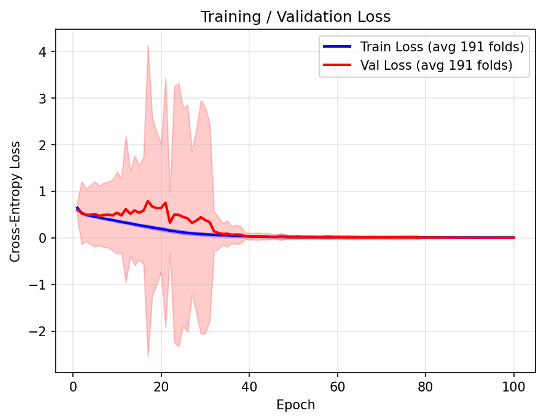
\includegraphics[width=\textwidth]{figures/2020_agcn_loss.png}
        \caption{2020 (LOOCV)}
        \label{fig:gcn_loss_2020}
    \end{subfigure}
    \hfill
    \begin{subfigure}[t]{0.32\textwidth}
        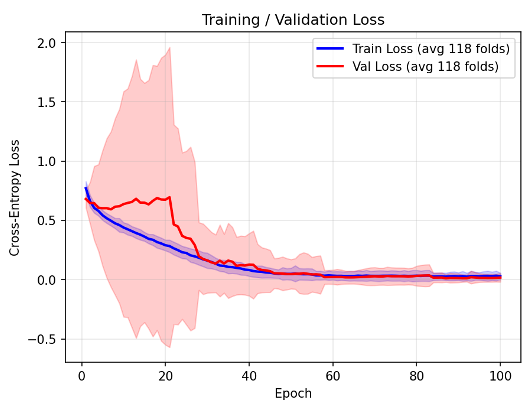
\includegraphics[width=\textwidth]{figures/2025_agcn_loss.png}
        \caption{2025 (LOOCV)}
        \label{fig:gcn_loss_2025}
    \end{subfigure}
    \hfill
    \begin{subfigure}[t]{0.32\textwidth}
        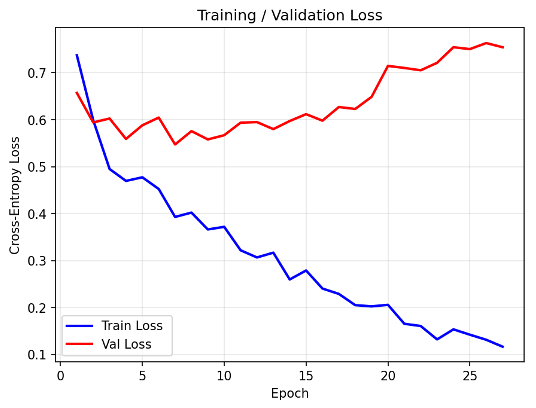
\includegraphics[width=\textwidth]{figures/cross_agcn_loss.png}
        \caption{Cross-cohort}
        \label{fig:gcn_loss_cross}
    \end{subfigure}
    \caption{Training and validation loss curves of AGCN.}
    \label{fig:gcn_loss_comparison}
\end{figure}

\begin{figure}[H]
    \centering
    \begin{subfigure}[t]{0.32\textwidth}
        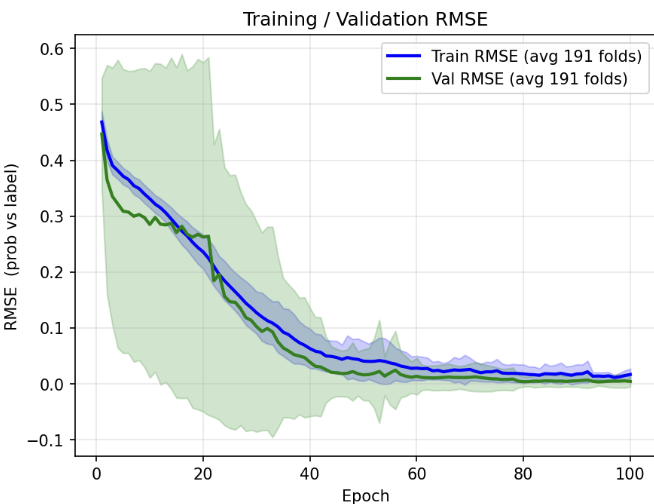
\includegraphics[width=\textwidth]{figures/2020_agcn_rmse.png}
        \caption{2020 (LOOCV)}
        \label{fig:gcn_rmse_2020}
    \end{subfigure}
    \hfill
    \begin{subfigure}[t]{0.32\textwidth}
        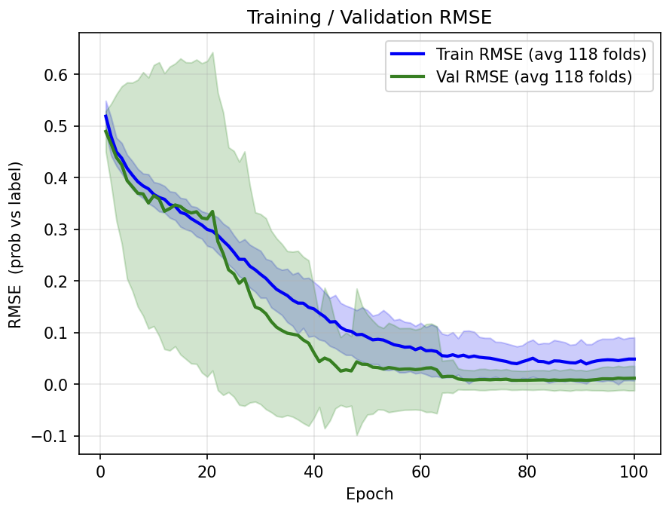
\includegraphics[width=\textwidth]{figures/2025_agcn_rmse.png}
        \caption{2025 (LOOCV)}
        \label{fig:gcn_rmse_2025}
    \end{subfigure}
    \hfill
    \begin{subfigure}[t]{0.32\textwidth}
        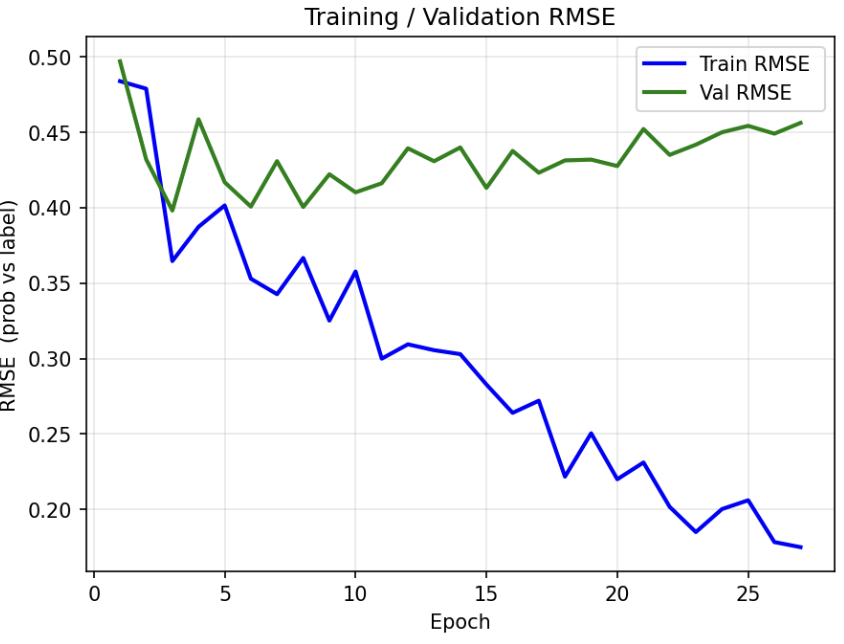
\includegraphics[width=\textwidth]{figures/cross_agcn_rmse.png}
        \caption{Cross-cohort}
        \label{fig:gcn_rmse_cross}
    \end{subfigure}
    \caption{Root Mean Square Error (RMSE) curves of AGCN across training epochs.}
    \label{fig:gcn_rmse_comparison}
\end{figure}

\subsection{Observation}

Within cohort, AGCN dominates every hand-crafted configuration from Experiments~2--4, reaching AUROCs of $0.98$ on both the 2020 and 2025 cohorts with accuracies of $0.92$--$0.93$ and F1-scores of $0.85$--$0.89$.

The loss and RMSE curves in Figs.~\ref{fig:gcn_loss_comparison} and~\ref{fig:gcn_rmse_comparison} provide important context for interpreting this result. Under LOOCV, each validation fold contains exactly one subject, so the per-fold validation loss is a single-sample measurement: when the model predicts that subject correctly the loss approaches zero, and when it fails the loss can be arbitrarily large. Averaged across all folds, both the mean training loss and the mean validation loss converge to near zero by epoch~100, and the validation RMSE likewise decays toward zero. This structural property of single-sample LOOCV means that the near-perfect within-cohort AUROC reflects the model's ability to classify each individual held-out subject after training on a near-complete cohort, rather than generalisation to a held-out distribution. The shaded variance bands further illustrate this: the 2020 cohort exhibits substantially wider per-fold variation (band spanning roughly $-2$ to $+4$ in the early epochs) than the 2025 cohort (band spanning roughly $0$ to $2$), consistent with the more heterogeneous video durations and recording conditions of the 2020 protocol relative to the standardised 30-second 2025 recordings.

In the cross-cohort transfer setting, the loss curves tell a qualitatively different story. The training loss decreases monotonically from $0.73$ to $0.12$, whereas the test-cohort loss rises steadily from approximately $0.60$ at epoch~1 to $0.75$ at the point of early stopping (epoch~$\approx 27$), yielding the classic diverging pattern of overfitting. The corresponding cross-cohort RMSE does not converge but oscillates and trends upward, ending near $0.46$, indicating that the model's probability estimates on the 2025 cohort become progressively less calibrated as training continues on the 2020 source distribution. Consequently, AGCN drops to an AUROC of $0.59$, an accuracy of $0.46$, and an F1-score of $0.40$, falling behind every hand-crafted configuration in Table~\ref{tab:gcn_cross_dataset}.

This sharp reversal from within-cohort to cross-cohort performance suggests that the adaptive graph topology learned from the 2020 training data may capture patterns that are specific to that cohort's distribution and do not generalise well to the 2025 recording protocol or patient population. One plausible contributing factor is that the graph adjacency is re-estimated from the node features of each training sample, so the discovered joint relationships may be sensitive to cohort-level differences in recording conditions, subject demographics, or movement characteristics; a sufficiently large distribution shift could invalidate the learned topology. Another likely factor is the small clinical dataset size, which provides limited headroom for the model to learn cohort-invariant representations: under LOOCV each fold trains on a near-complete cohort, favouring memorisation over generalisation. Taken together, these factors offer a plausible account of why AGCN underperforms the hand-crafted baselines in cross-cohort evaluation, although the relative contribution of each factor cannot be isolated from this experiment alone.

% !TeX root = ../main.tex

\chapter{Conclusions and Future Work}
\label{chap:conclusion}

\section{Conclusions}

This thesis investigated the binary classification of Parkinson's Disease from short hand-rotation videos recorded with everyday smartphones or tablets. A four-stage pipeline was constructed, consisting of MediaPipe-based 3D hand keypoint extraction, hand-crafted kinematic features (frequency, clarity, and four complementary amplitude representations), three feature-selection strategies (ANOVA F-value, L1-regularized Logistic Regression, and XGBoost gain-based importance), and a comparison of four downstream classifiers (Logistic Regression, Random Forest, XGBoost, and AGCN). Five experiments were carried out on two NTUH clinical cohorts (the 2020 and 2025 cohorts), with both LOOCV within-cohort validation and 2020-to-2025 cross-cohort transfer evaluation.

The principal findings are summarized as follows:

\begin{enumerate}
    \item \textbf{The motor reserve phenomenon makes left-hand features highly impactful for PD prediction.} Across both cohorts, left-hand-only models consistently outperformed right-hand-only and bilateral models, and the top-10 features were dominated by the left hand (25:5 and 19:11 in favour of the left hand). This is qualitatively consistent with the motor reserve hypothesis: in a predominantly right-handed cohort, the non-dominant left hand carries less compensatory reserve and therefore reveals bradykinesia more clearly during the pronation-supination task.

    \item \textbf{Adding pairwise joint-correlation features improves performance only marginally.} Augmenting the bilateral feature set with explicit pairwise Pearson correlation features did not consistently outperform the strongest single-side baseline. Within cohort, the correlation-augmented configurations were on par with or slightly worse than the left-hand XGB Importance baseline; in cross-cohort transfer, AUROC improved only marginally (from $0.65$--$0.66$ to $0.68$) and without a stable improvement in accuracy or F1-score.

    \item \textbf{AGCN markedly improves within-cohort performance but does not transfer.} The AGCN reached AUROCs of $0.97$--$0.98$ within each cohort under LOOCV. In cross-cohort transfer, however, AUROC collapsed to $0.53$--$0.62$, comparable to or worse than the best hand-crafted feature configurations.

    \item \textbf{Adaptive graph topologies are highly dependent on the training distribution.} Because the AGCN learns its joint-wise adjacency from the training cohort itself, the discovered graph topology does not transfer across years: the structure that is optimal for the 2020 protocol and population is no longer optimal for the 2025 protocol and population.

    \item \textbf{Small clinical datasets exacerbate the domain-shift problem.} Under LOOCV, every fold trains on a near-identical distribution, so even high-capacity models such as AGCN can fit it well. Under cross-cohort transfer, however, the limited sample size leaves no headroom for the model to learn invariant patterns, and the resulting overfitting magnifies the domain shift between the 2020 and 2025 cohorts.
\end{enumerate}

\section{Future Work}

Based on the limitations and findings above, three directions are identified for future investigation:

\begin{enumerate}
    \item \textbf{Continue data collection to evaluate cross-year stability.} Larger, longitudinally collected cohorts would enable a more reliable estimate of cross-year generalization and would create headroom for higher-capacity models such as AGCN to overcome small-sample overfitting.

    \item \textbf{Lightweight the model and deploy it at the edge.} Because MediaPipe is designed for mobile hardware, the entire feature-extraction and classification pipeline can in principle be lightweighted (e.g., via quantization or distillation) and deployed on the user's device. This would enable real-time, at-home PD monitoring without the need for a server round trip.

    \item \textbf{Explore multi-modal large models combining hand gesture, gait, and voice.} PD affects multiple motor and non-motor modalities. Combining hand-rotation video with gait video and voice recordings within a unified multi-modal large model is a promising direction: the complementarity of these modalities, together with the benefits of foundation-model pretraining, could mitigate the small-cohort overfitting that limited the AGCN in this study.
\end{enumerate}


% 參考文獻
% References
\refmatter
\bibliographystyle{unsrt}
\bibliography{back/references}

\end{document}
